Laboratorní měření bylo provedeno celkem na 20 kombinacích modelu respiračního systému. Postupně byly vyměněny dvě velikosti nádob, 3 délky plastové trubice a 3 velikosti parabolického odporu. Přístroj měří několik veličin: reaktanci, rezistenci, objem, rezonanční frekvenci a $COH_{3}$.. Tato práce se popisuje změnu rezistance a reaktance vůči různým komponentům.  

 
\subsection{Rezistance}

Výsledky pro menší nádobu tj. \SI{35}{L} vyšly ve většině případů s menší odchylkou než výsledky měření s 54 litrovou nádobou. Pro odpor 20 vyšla rezistence cca o 0,5 větší u nádoby 35L. Hodnoty rezistence pro odpor 5 vyšly naopak vyšší pro nádobu s menším objemem. 

Pří měření s delší plastovou trubicí vyšly také výsledky s menší odchylkou. 
Při zvětšení inertance, neboli použití delší plastové trubice se rezistence ce u všech velikostí průtočného odporu cca o  $\SI{0,5}{ cm\cdot H_{2}O \cdot s/L} $ zvýší. 
Při zvýšení poddajnosti, tj. při použití nádoby s  větším objemem rezistence o cca  $\SI{0,5}{ cm\cdot H_{2}O \cdot s/L} $  klesne. 
Při použití Rp 20 je rezistence o také cca  $\SI{0,5}{ cm\cdot H_{2}O \cdot s/L} $  vyšší než u Rp 5 a Rp 50. 

\subsection{Reaktance}

Čím víc se snižovala inertance, tj. čím kratší byla plastová trubice tím víc klesala i reaktance. Při větší poddajnosti se reaktance zvedla. Stejně jako u rezistence byla i reaktance nejvyšší při použití Rp 20. Odchylky pro měření s větší i menší nádobou jsou podobné. 


Měřena byla především rezistence, reaktance, rezonanční frekvence, objem a $COH_{3}$. 

\begin{figure}[ht]
	\label{img:pic_rezistance_delka_20_cm_nadoba_35_L}
	\begin{center}
		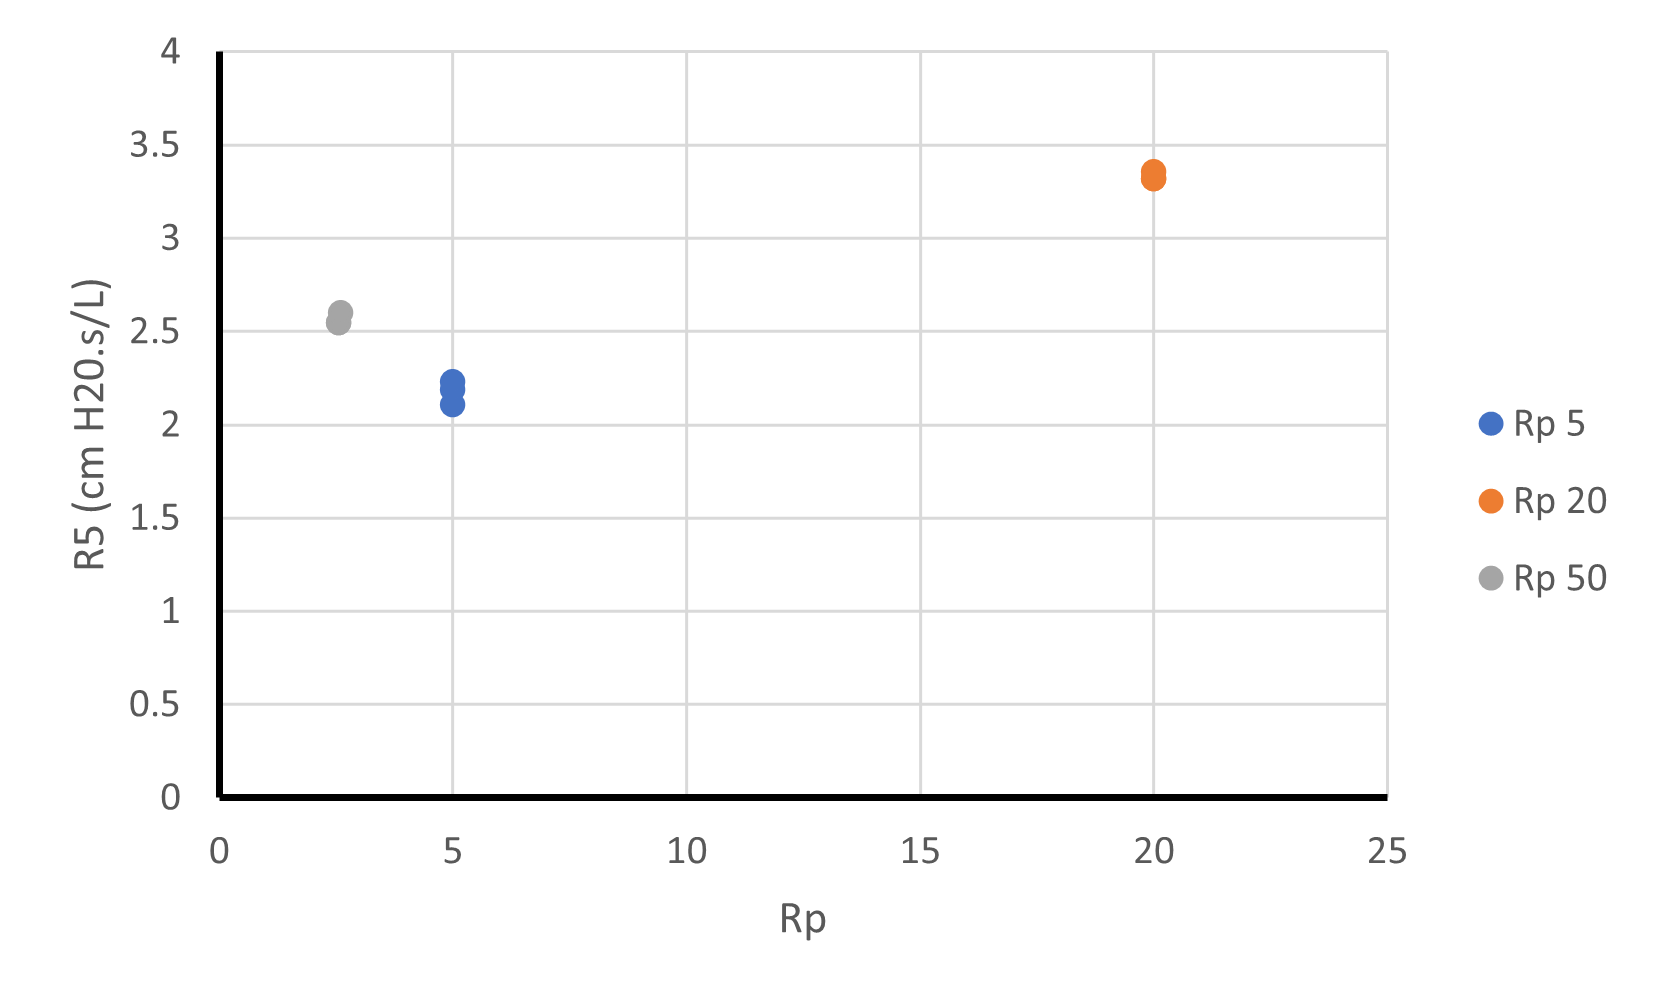
\includegraphics[width=1\textwidth]{rezistance_delka_20_cm_nadoba_35_L}
		\caption{Délka \SI{20}{cm}, nádoba~35L}
	\end{center}
\end{figure}

\begin{figure}[ht]
	\label{img:pic_rezistance_delka_20_cm_nadoba_54_L}
	\begin{center}
		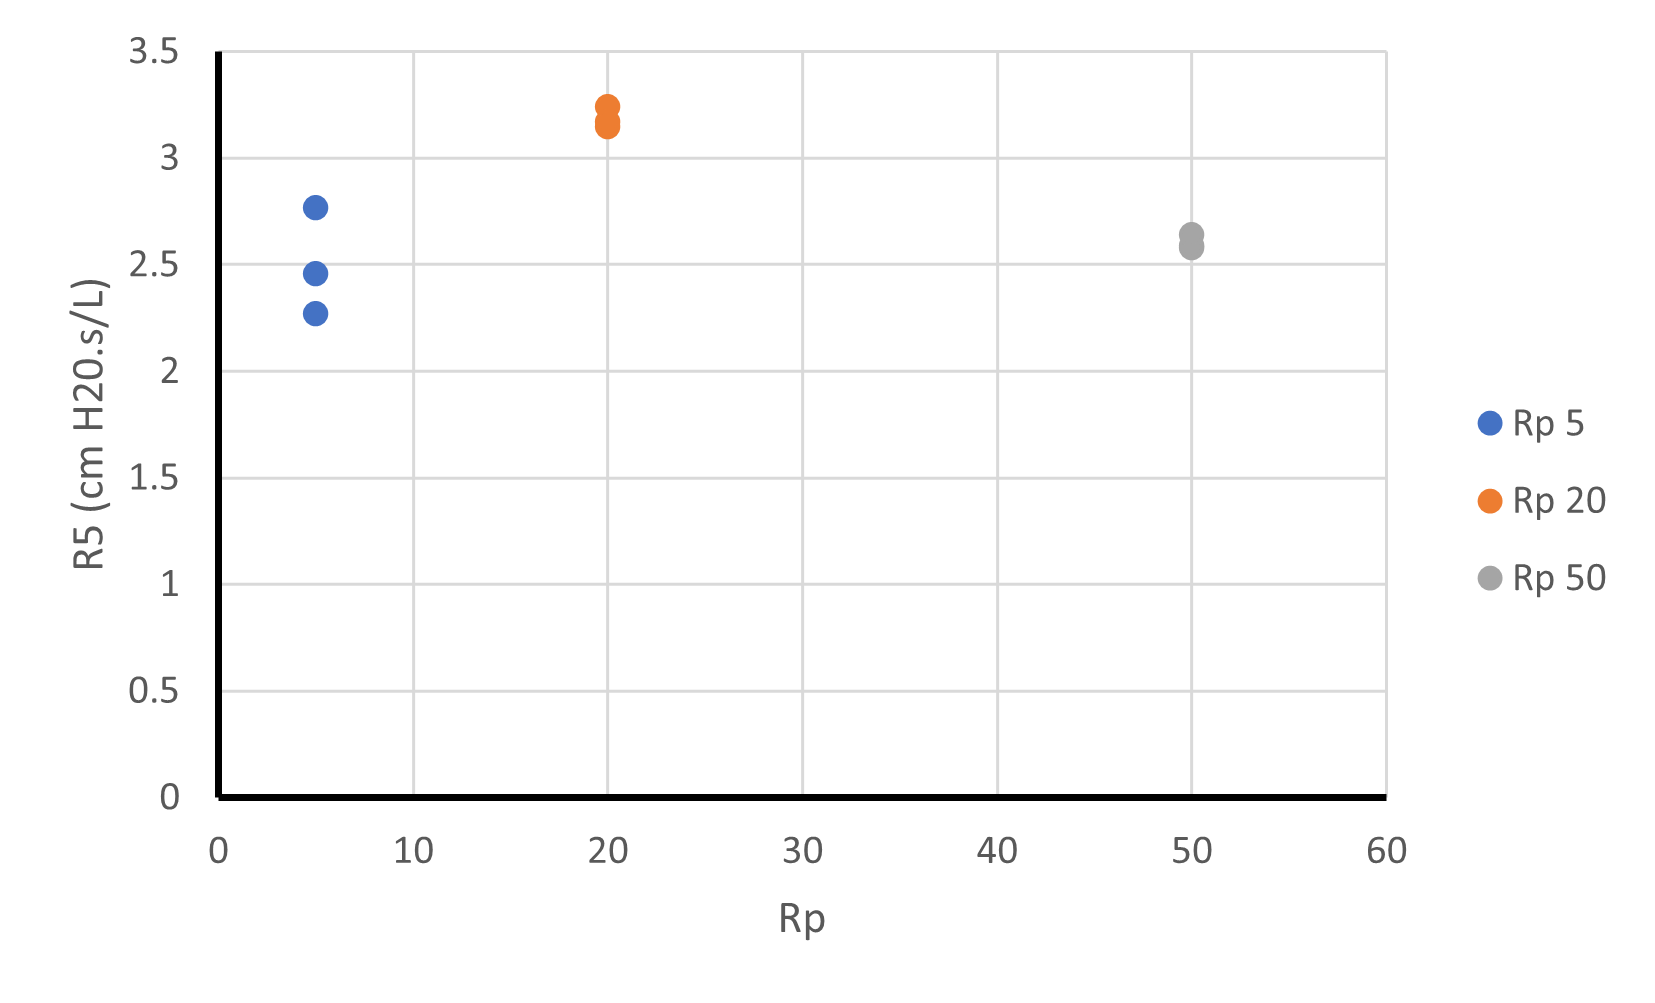
\includegraphics[width=1\textwidth]{rezistance_delka_20_cm_nadoba_54_L}
		\caption{Délka \SI{20}{cm}, nádoba~54L}
	\end{center}
\end{figure}

\begin{figure}[ht]
	\label{img:pic_rezistance_delka_40_cm_naboba_54_L}
	\begin{center}
		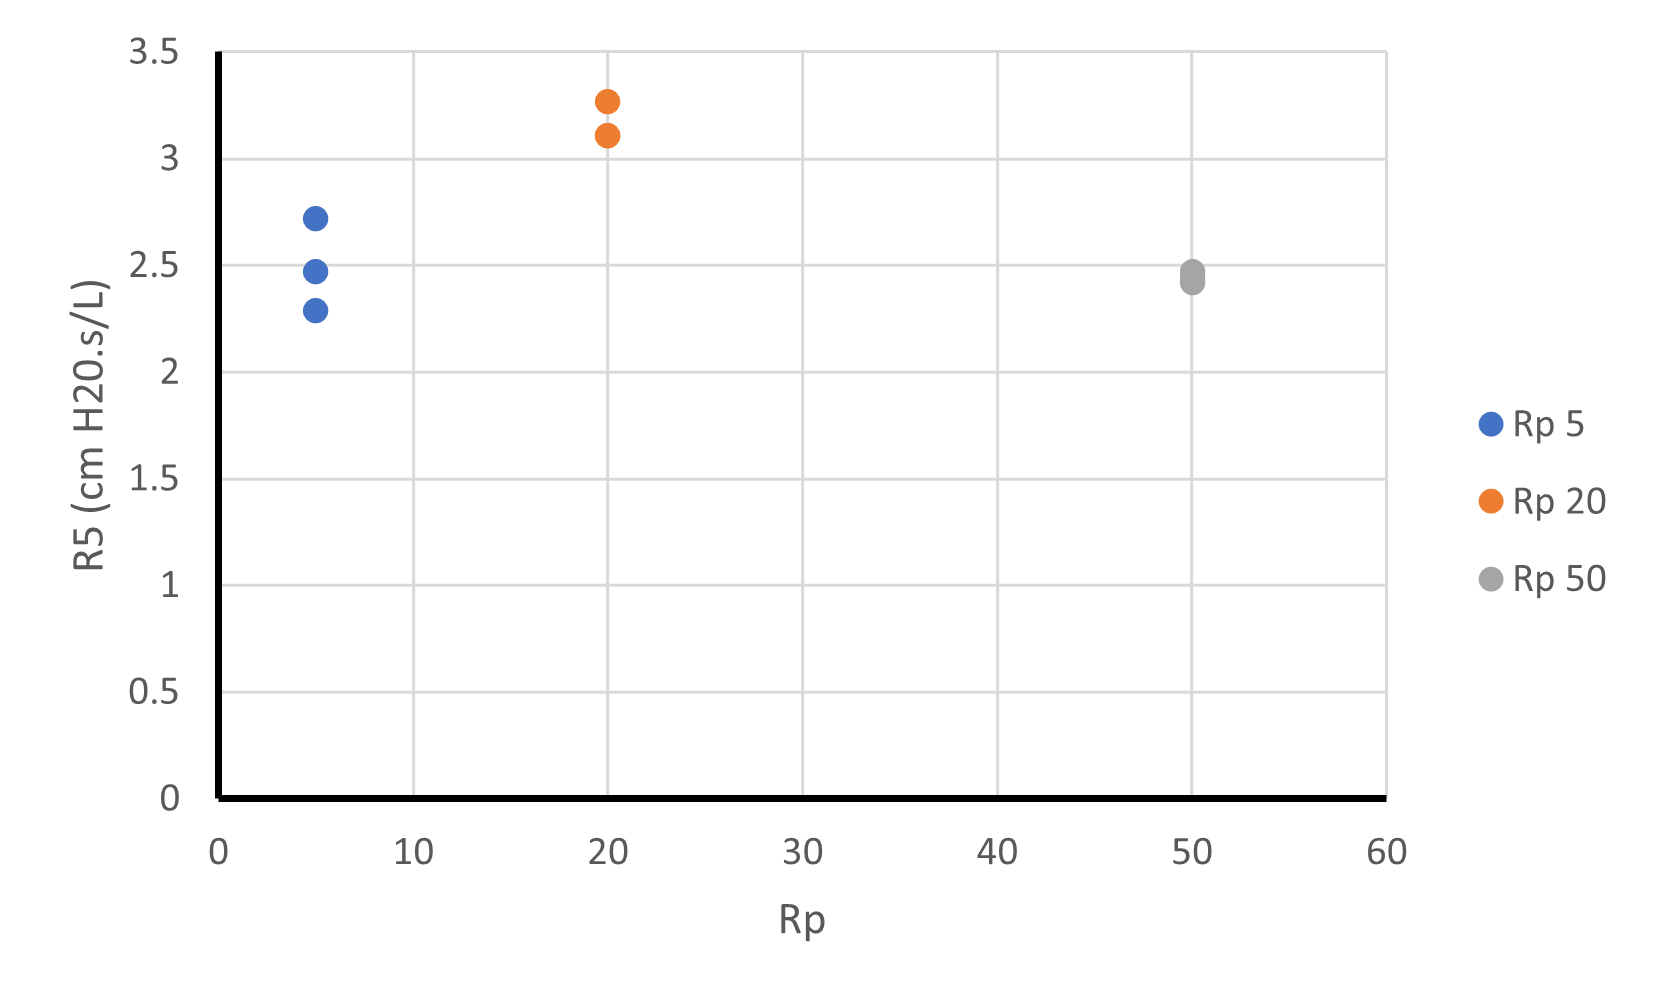
\includegraphics[width=1\textwidth]{rezistance_delka_40_cm_naboba_54_L}
		\caption{Délka \SI{40}{cm}, nádoba~54L}
	\end{center}
\end{figure}

\begin{figure}[ht]
	\label{img:pic_rezistance_delka_40_cm_nadoba_35_L}
	\begin{center}
		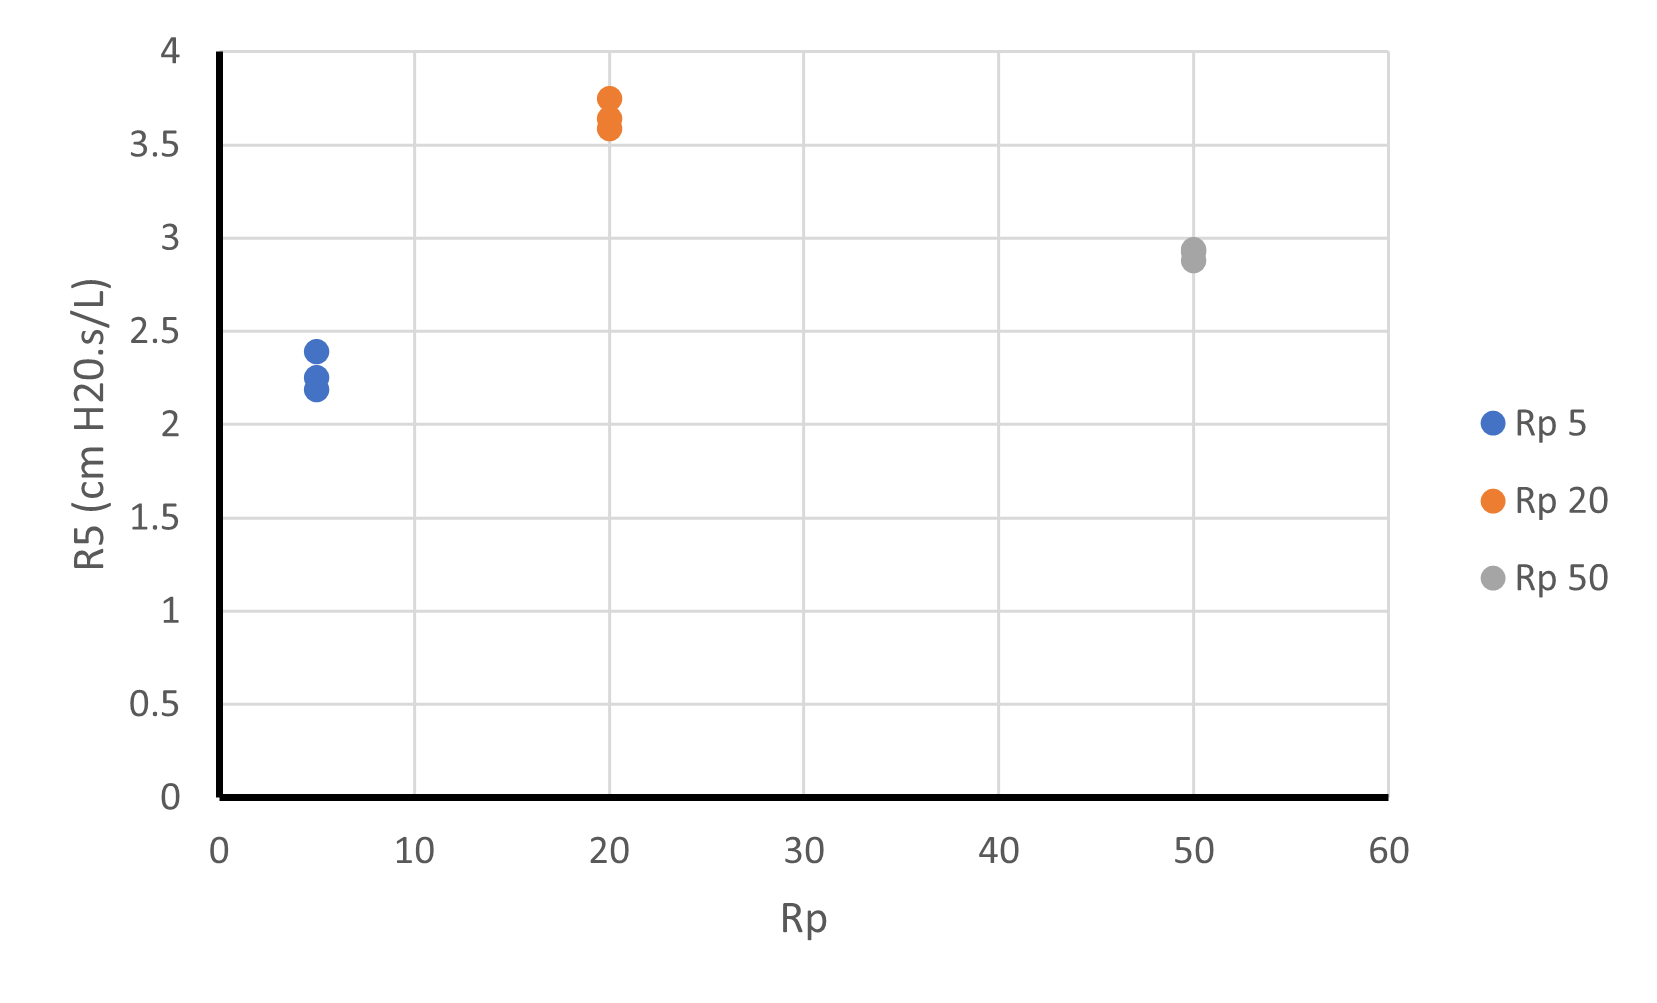
\includegraphics[width=1\textwidth]{rezistance_delka_40_cm_nadoba_35_L}
		\caption{Délka \SI{40}{cm}, nádoba~35L}
	\end{center}
\end{figure}

\begin{figure}[ht]
	\label{img:pic_rezistance_delka_60_cm_nadoba_35_L}
	\begin{center}
		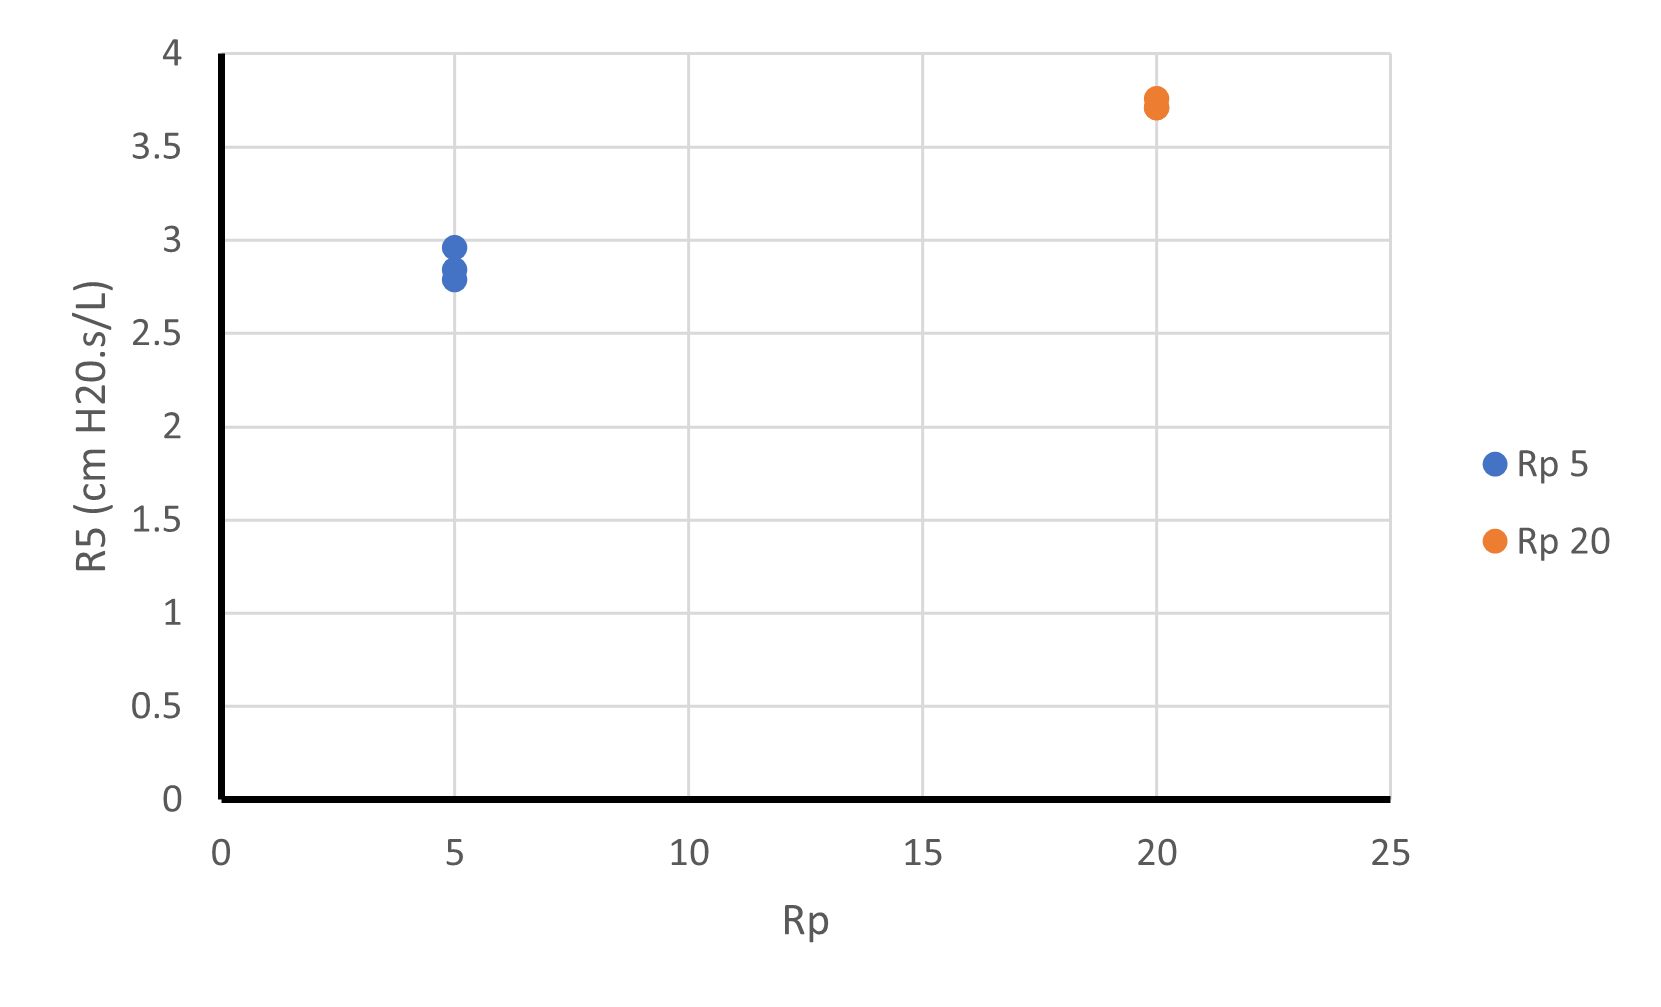
\includegraphics[width=1\textwidth]{rezistance_delka_60_cm_nadoba_35_L}
		\caption{Délka \SI{60}{cm}, nádoba~35L}
	\end{center}
\end{figure}

\begin{figure}[ht]
	\label{img:pic_rezistance_délka_60_cm_nádoba_54_L}
	\begin{center}
		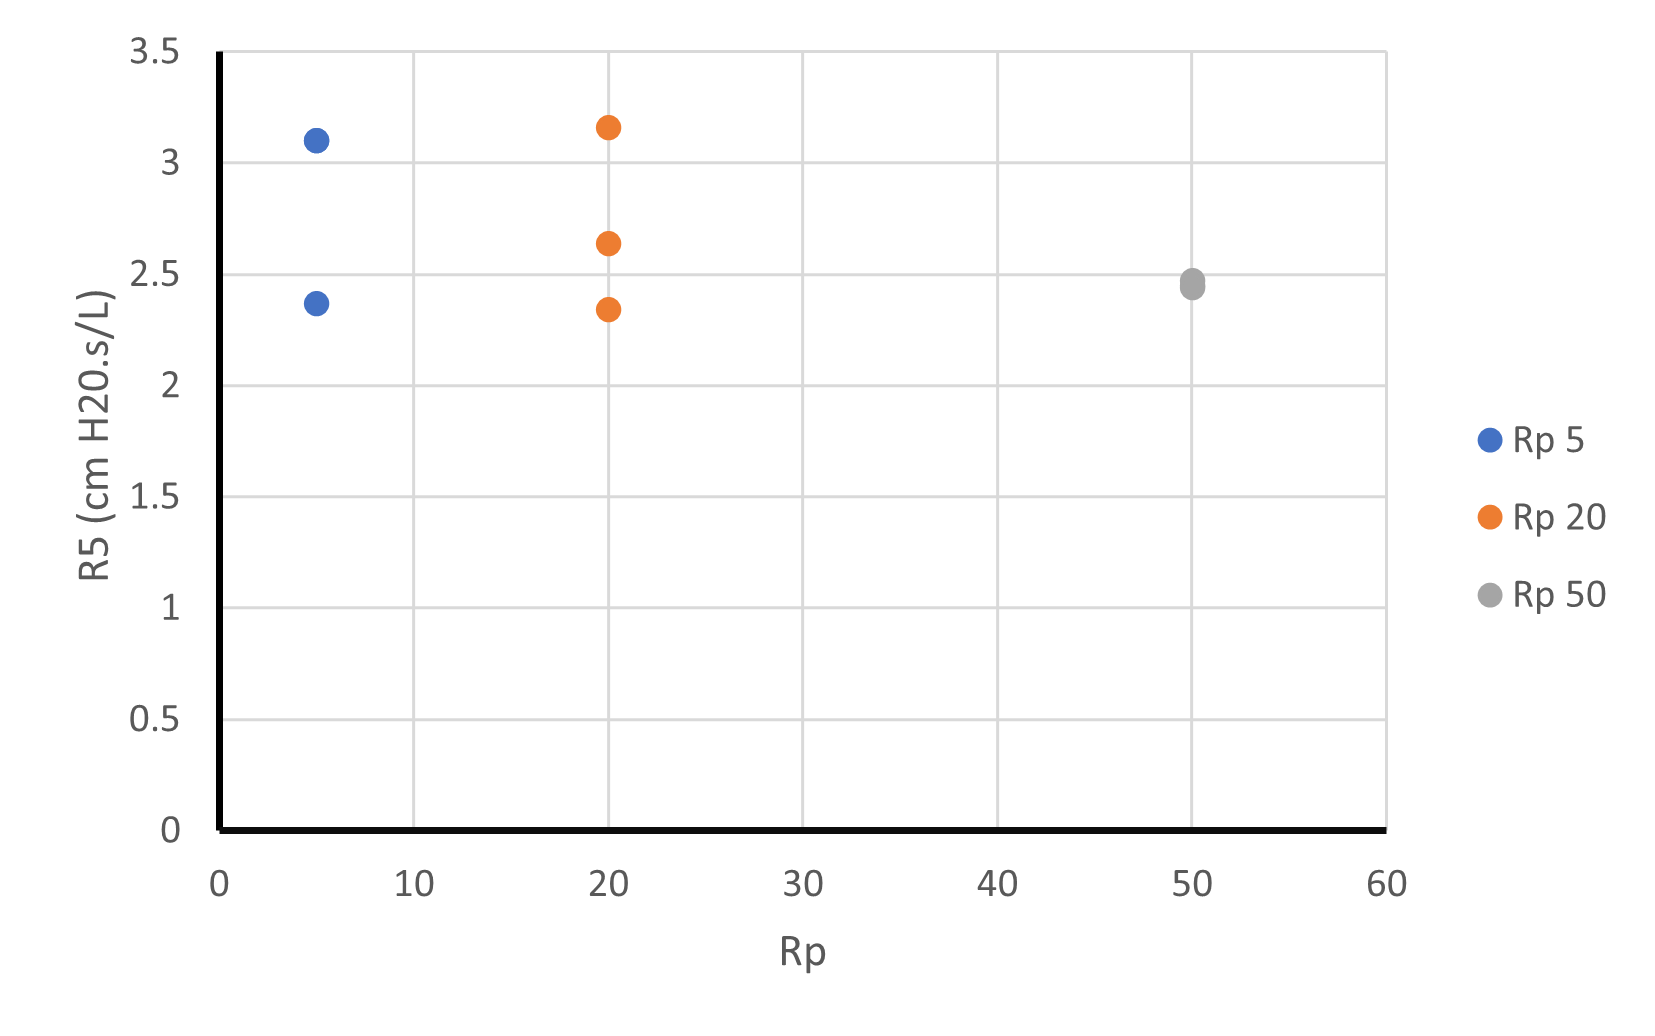
\includegraphics[width=1\textwidth]{rezistance_délka_60_cm_nádoba_54_L}
		\caption{Délka \SI{60}{cm}, nádoba~54L}
	\end{center}
\end{figure}


\begin{figure}[ht]
	\label{img:pic_rezistance_odpor_20_delka_20_cm}
	\begin{center}
		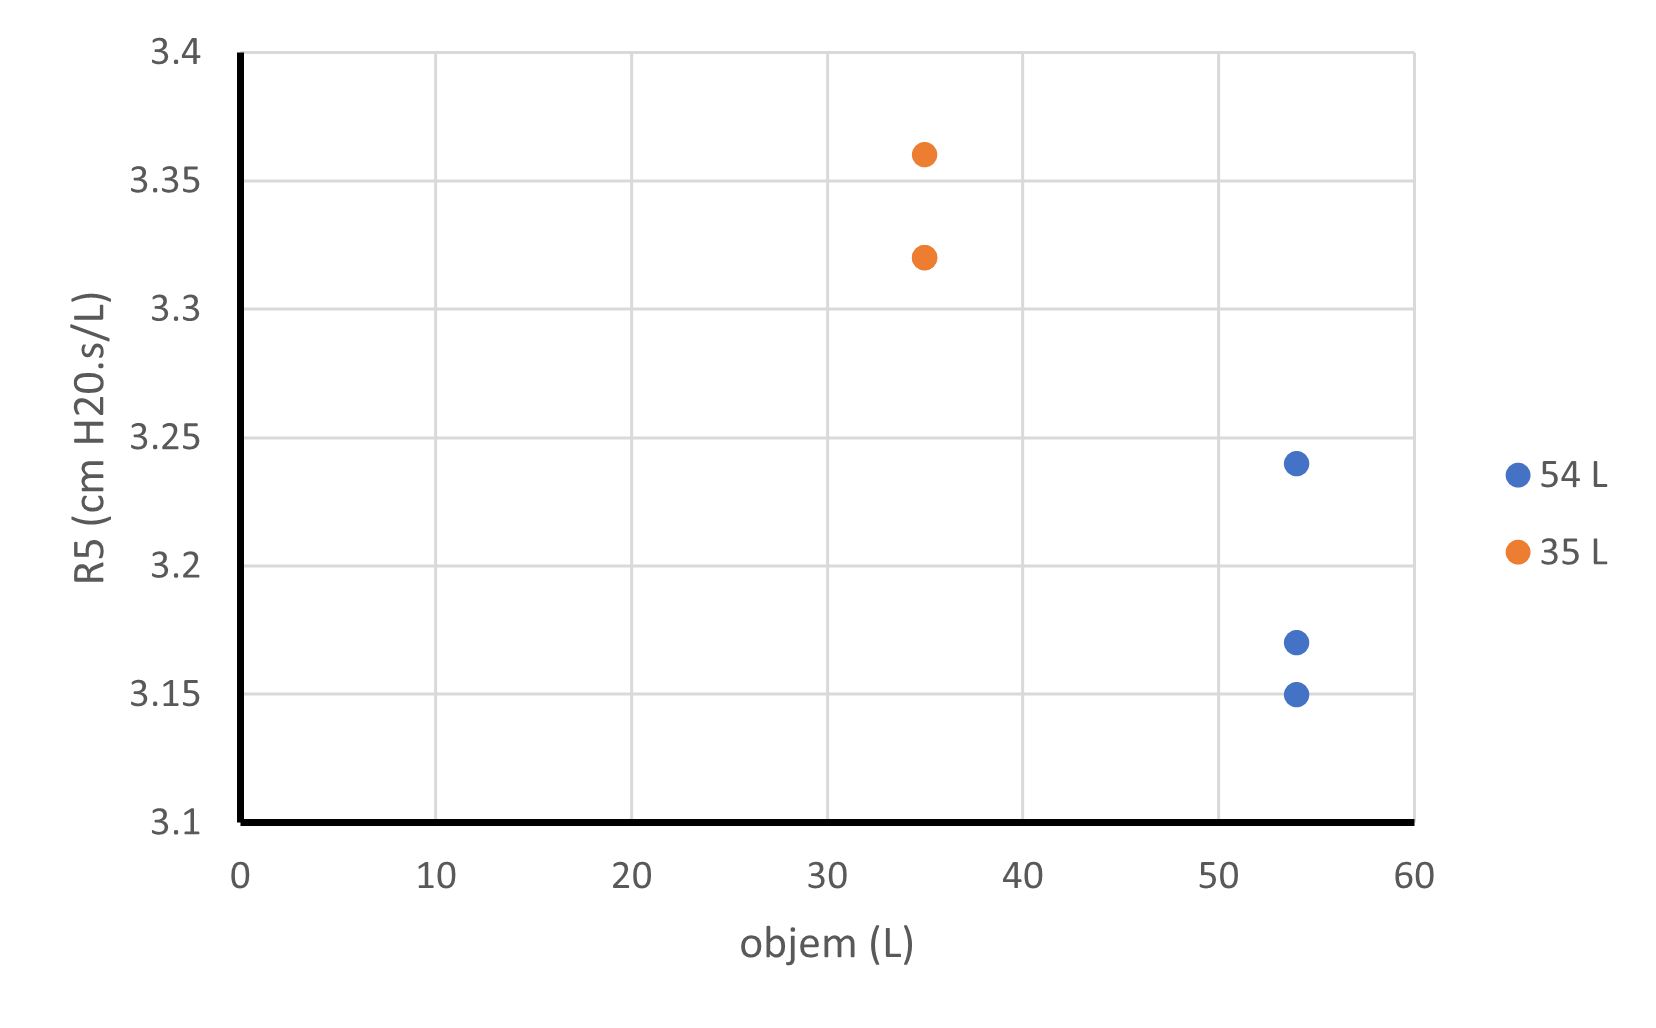
\includegraphics[width=1\textwidth]{rezistance_odpor_20_delka_20_cm}
		\caption{Délka \SI{20}{cm}, odpor~20}
	\end{center}
\end{figure}


\begin{figure}[ht]
	\label{img:pic_rezistance_odpor_20_delka_40_cm}
	\begin{center}
		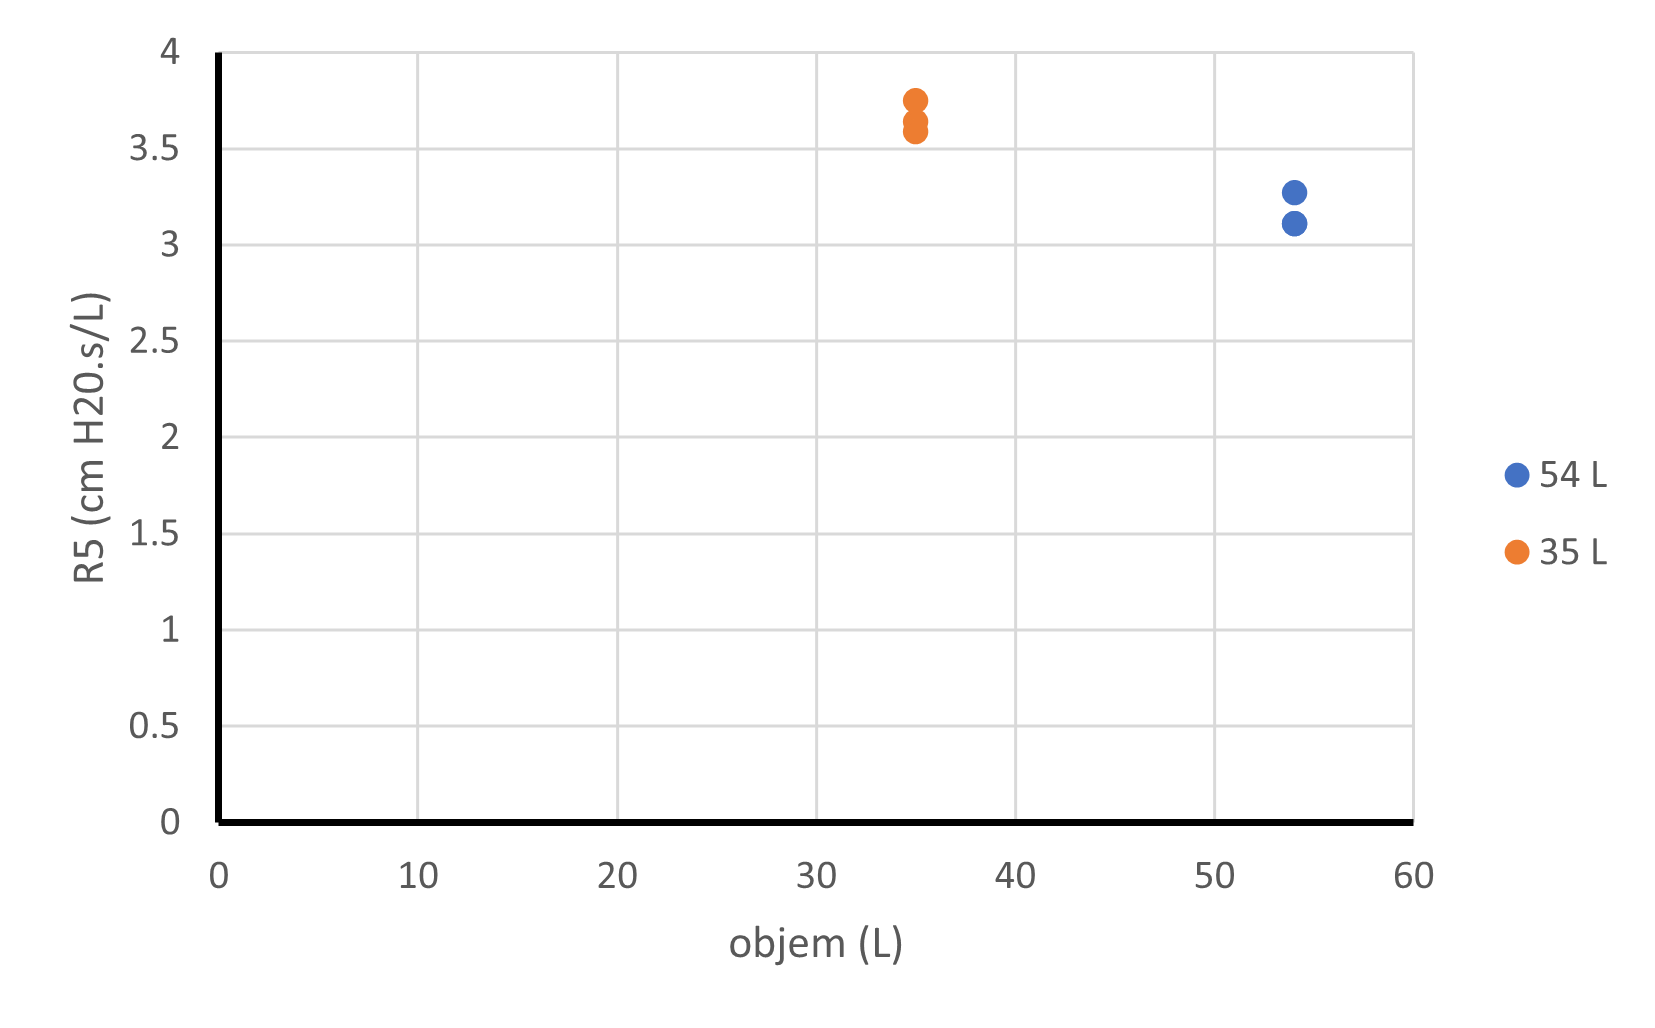
\includegraphics[width=1\textwidth]{rezistance_odpor_20_delka_40_cm}
		\caption{Délka \SI{40}{cm}, odpor~20}
	\end{center}
\end{figure}

\begin{figure}[ht]
	\label{img:pic_rezistance_odpor_20_delka_60_cm}
	\begin{center}
		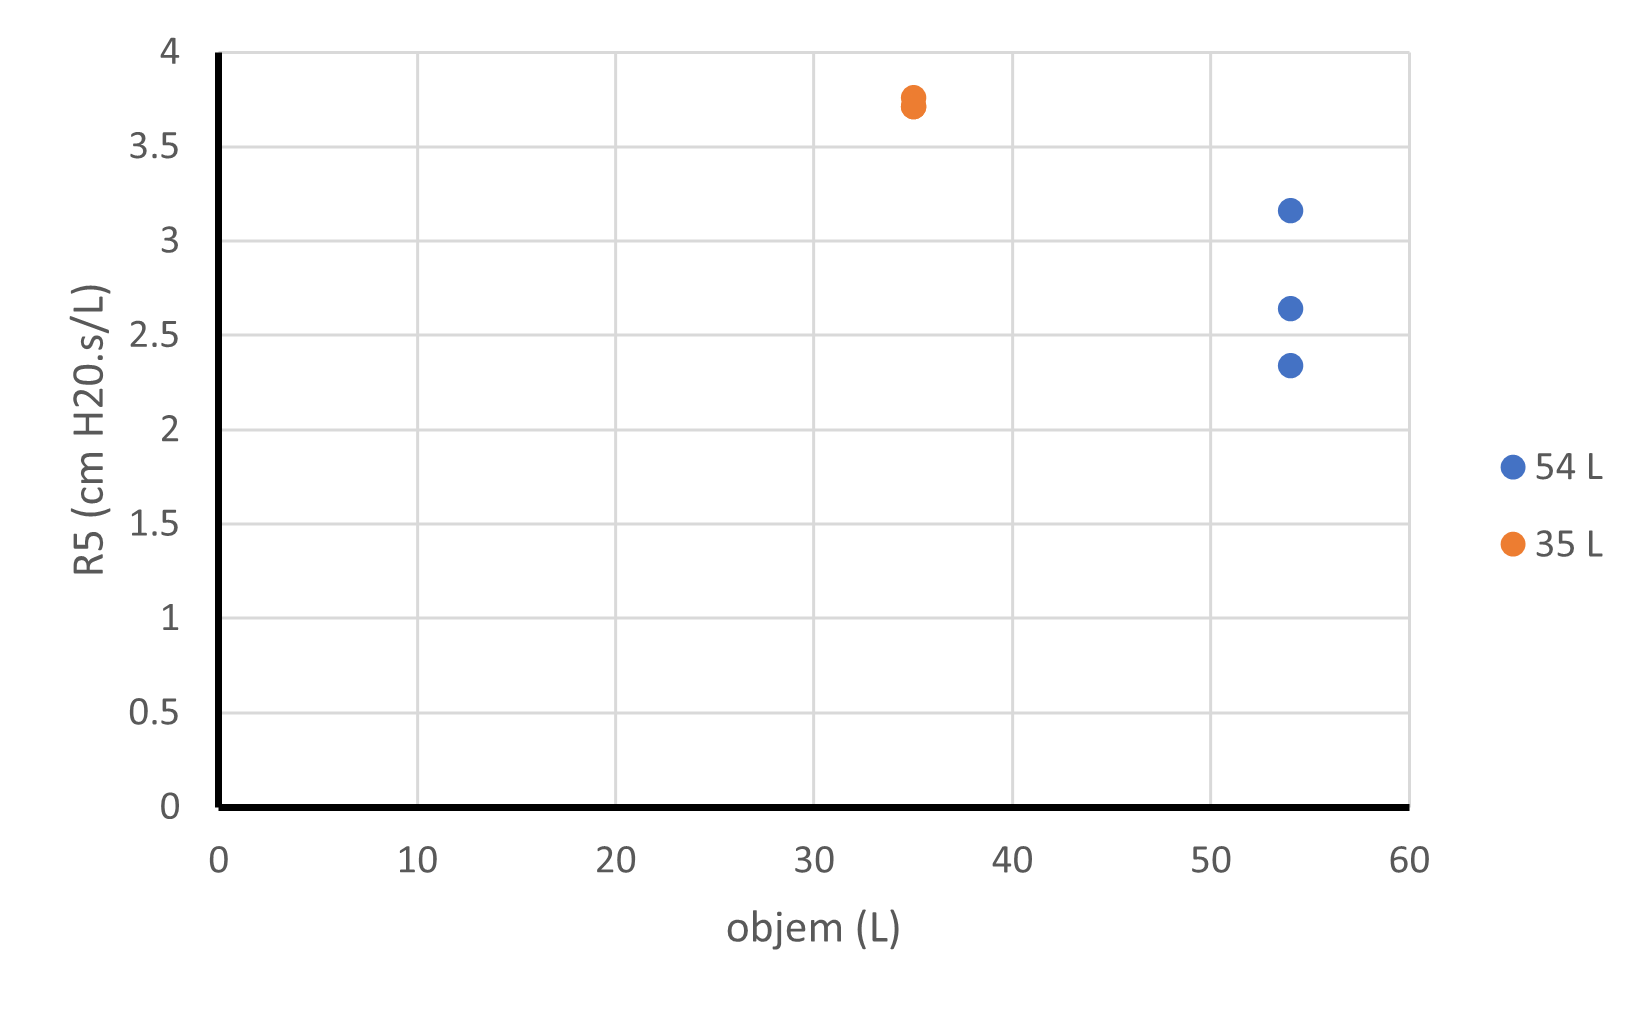
\includegraphics[width=1\textwidth]{rezistance_odpor_20_delka_60_cm}
		\caption{Délka \SI{60}{cm}, odpor~20}
	\end{center}
\end{figure}

\begin{figure}[ht]
	\label{img:pic_rezistance_odpor_5_delka_20_cm}
	\begin{center}
		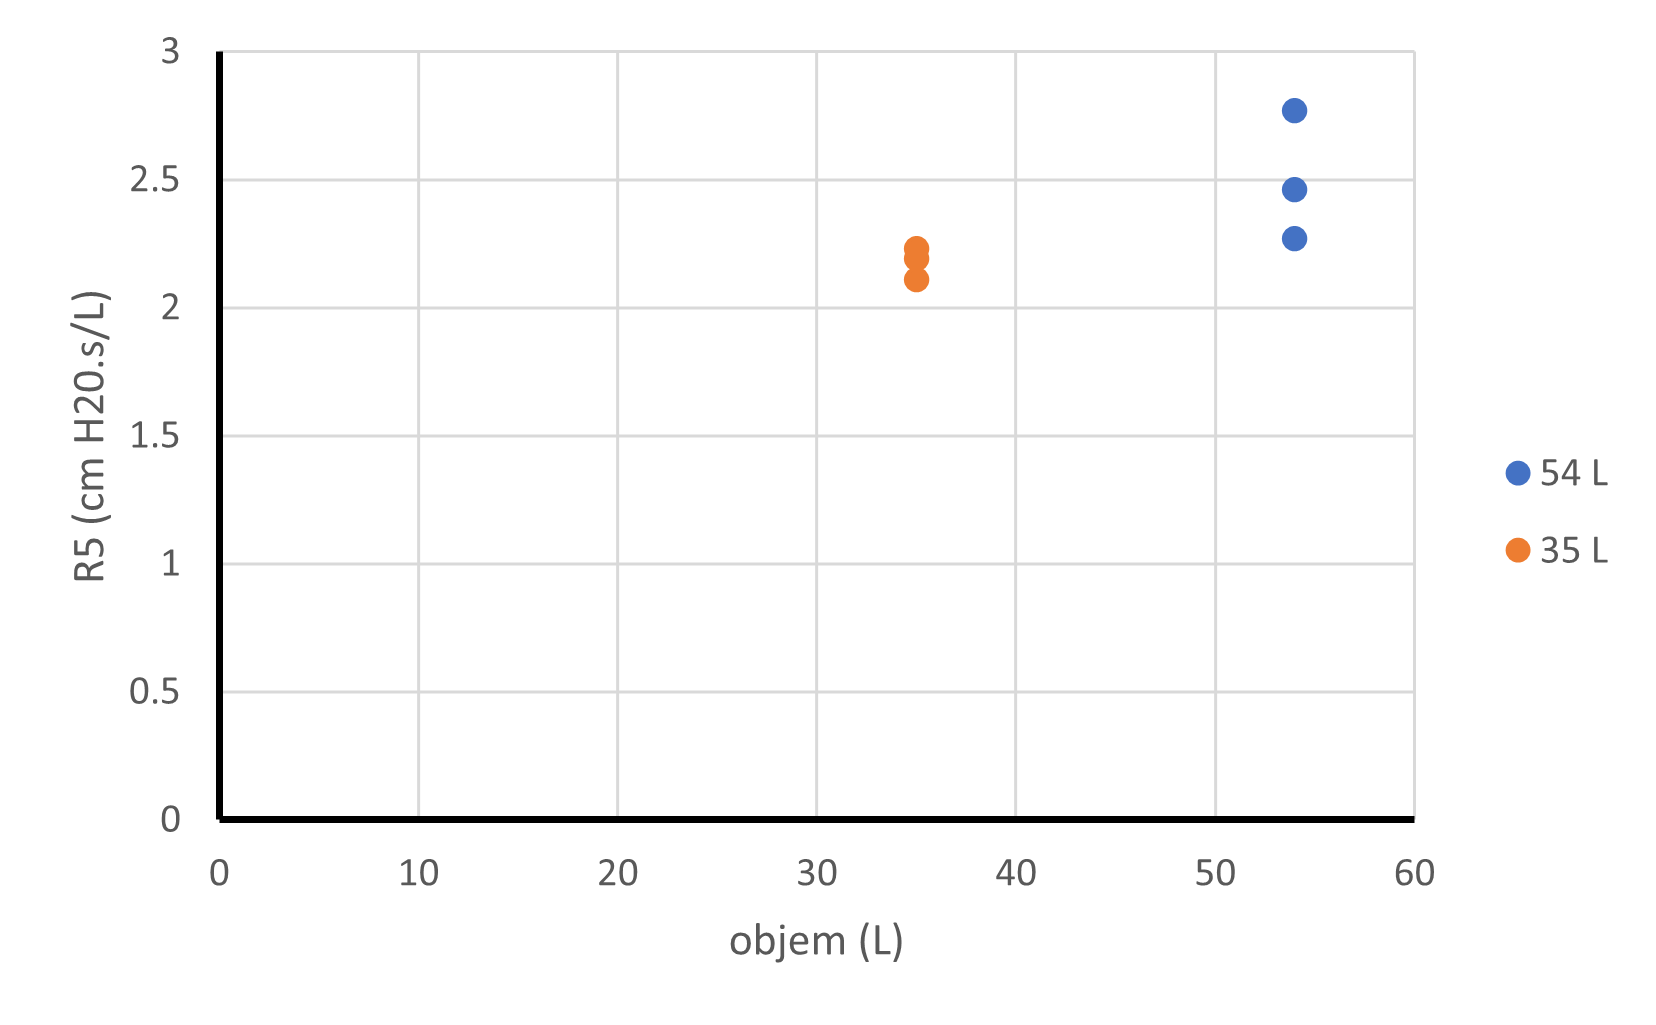
\includegraphics[width=1\textwidth]{rezistance_odpor_5_delka_20_cm}
		\caption{Délka \SI{20}{cm}, odpor~5}
	\end{center}
\end{figure}

\begin{figure}[ht]
	\label{img:pic_rezistance_odpor_5_delka_40_cm}
	\begin{center}
		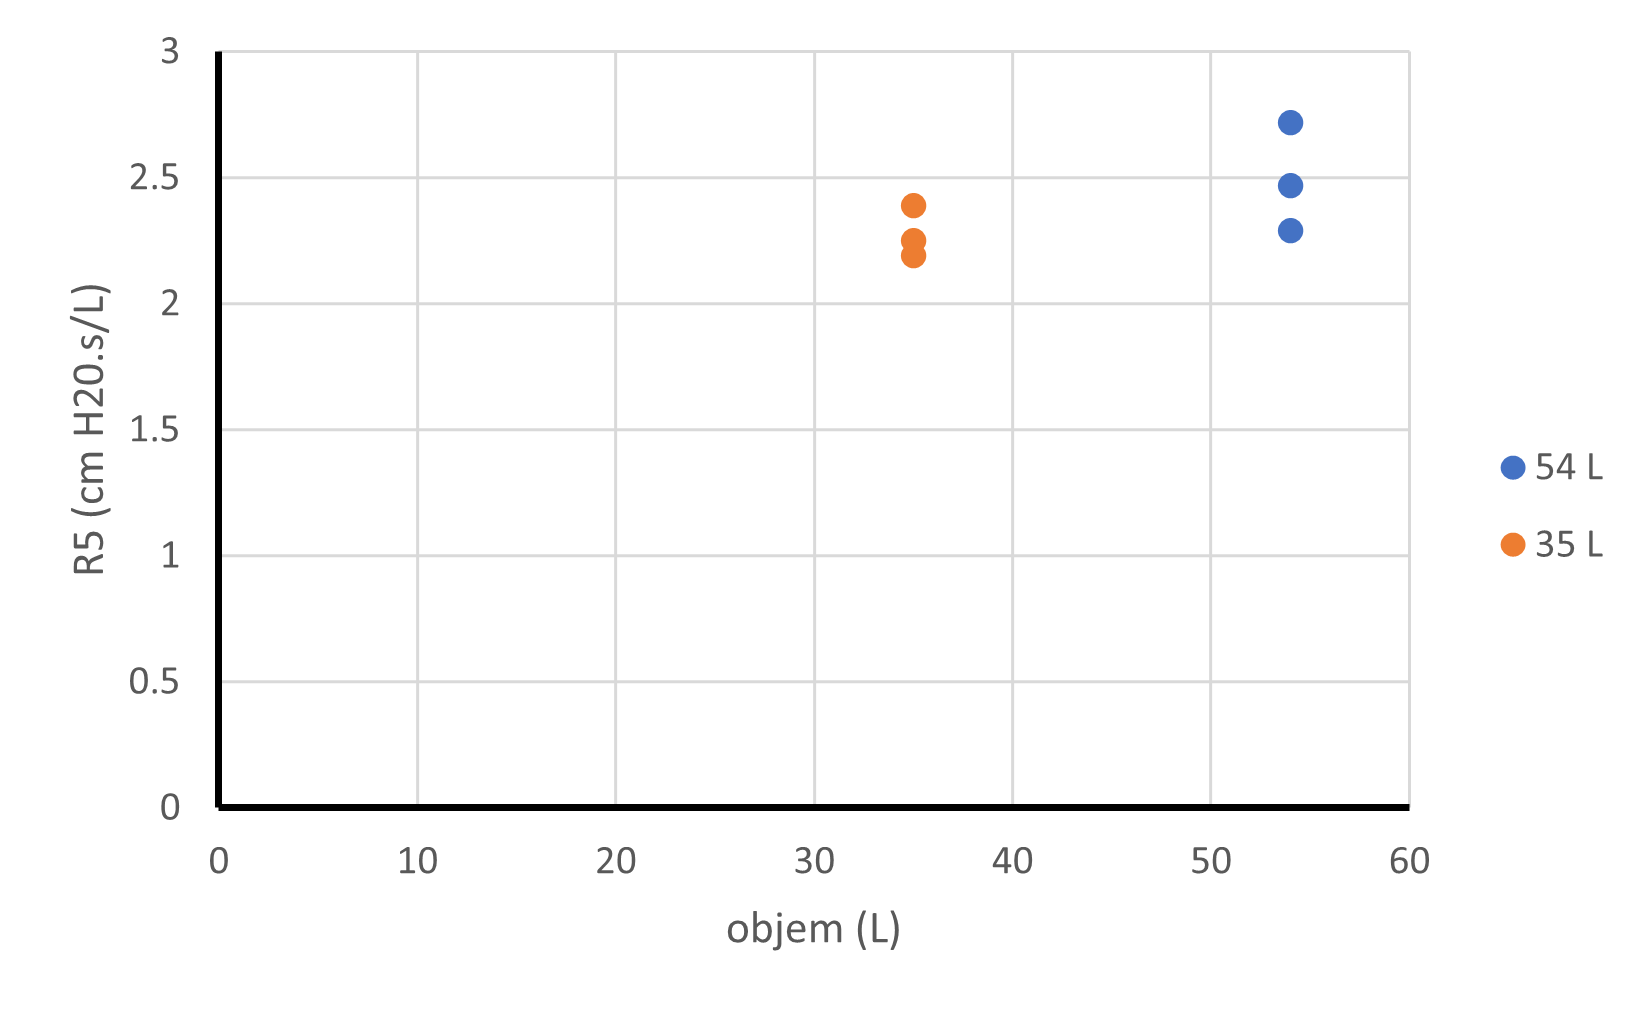
\includegraphics[width=1\textwidth]{rezistance_odpor_5_delka_40_cm}
		\caption{Délka \SI{40}{cm}, odpor~5}
	\end{center}
\end{figure}

\begin{figure}[ht]
	\label{img:pic_rezistance_odpor_5_delka_60_cm}
	\begin{center}
		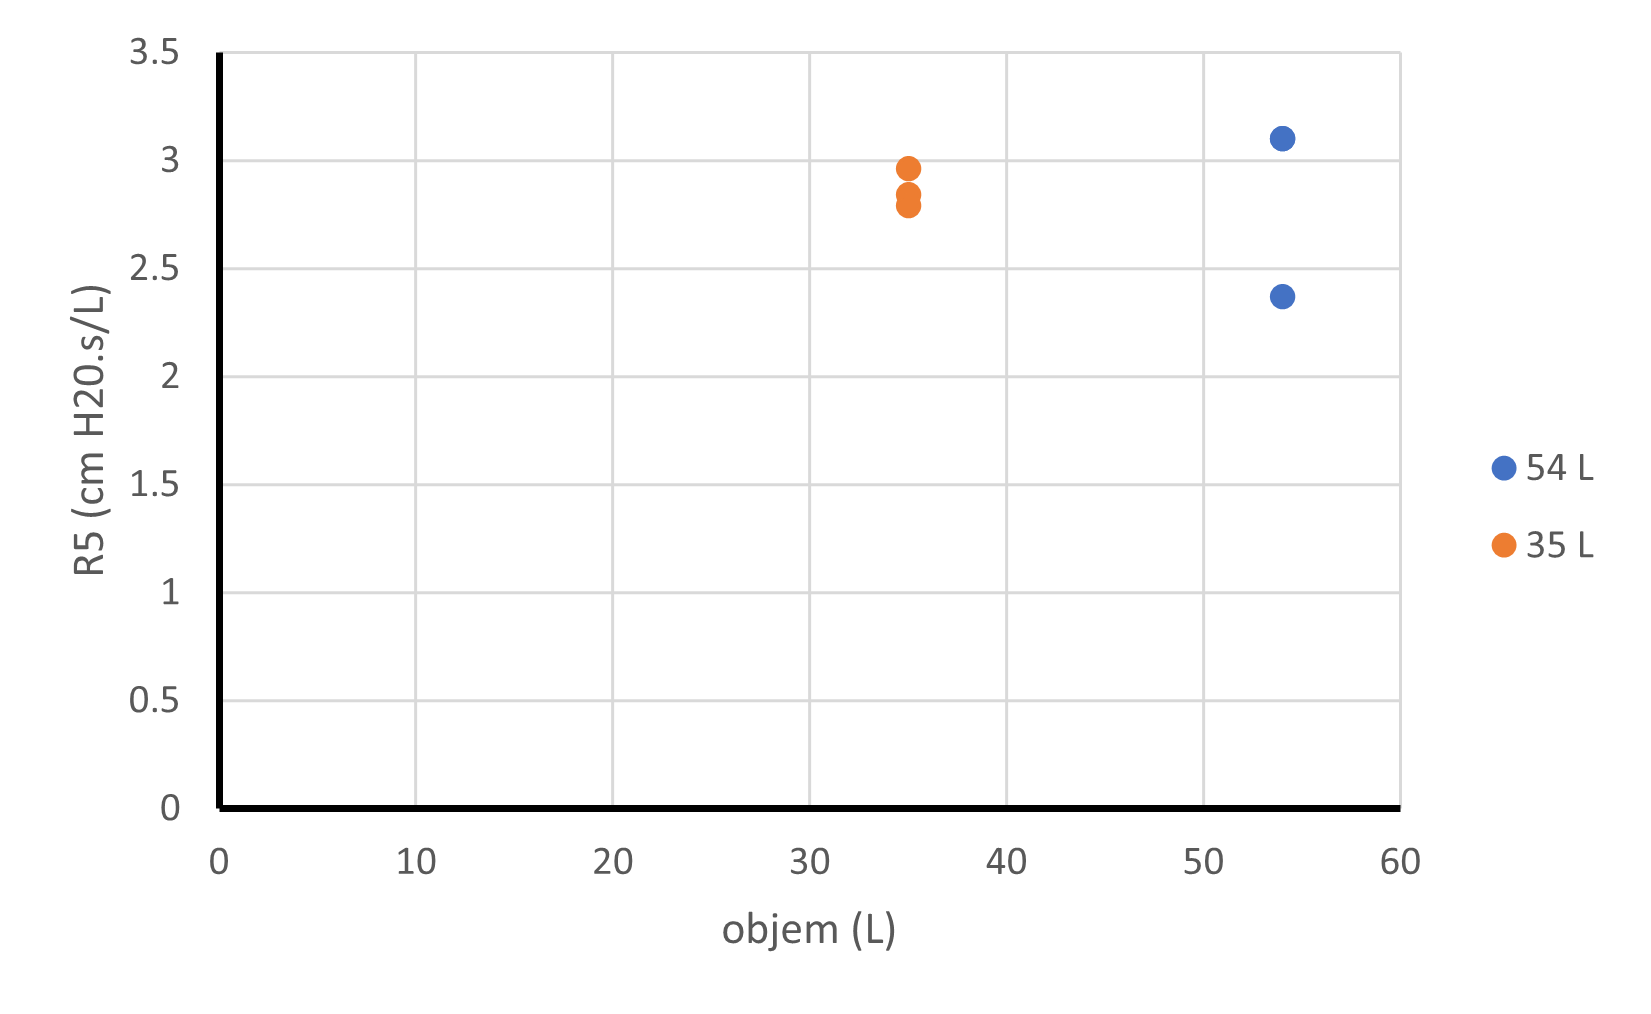
\includegraphics[width=1\textwidth]{rezistance_odpor_5_delka_60_cm}
		\caption{Délka \SI{60}{cm}, odpor~5}
	\end{center}
\end{figure}

\begin{figure}[ht]
	\label{img:pic_rezistance_odpor_50_delka_20_cm}
	\begin{center}
		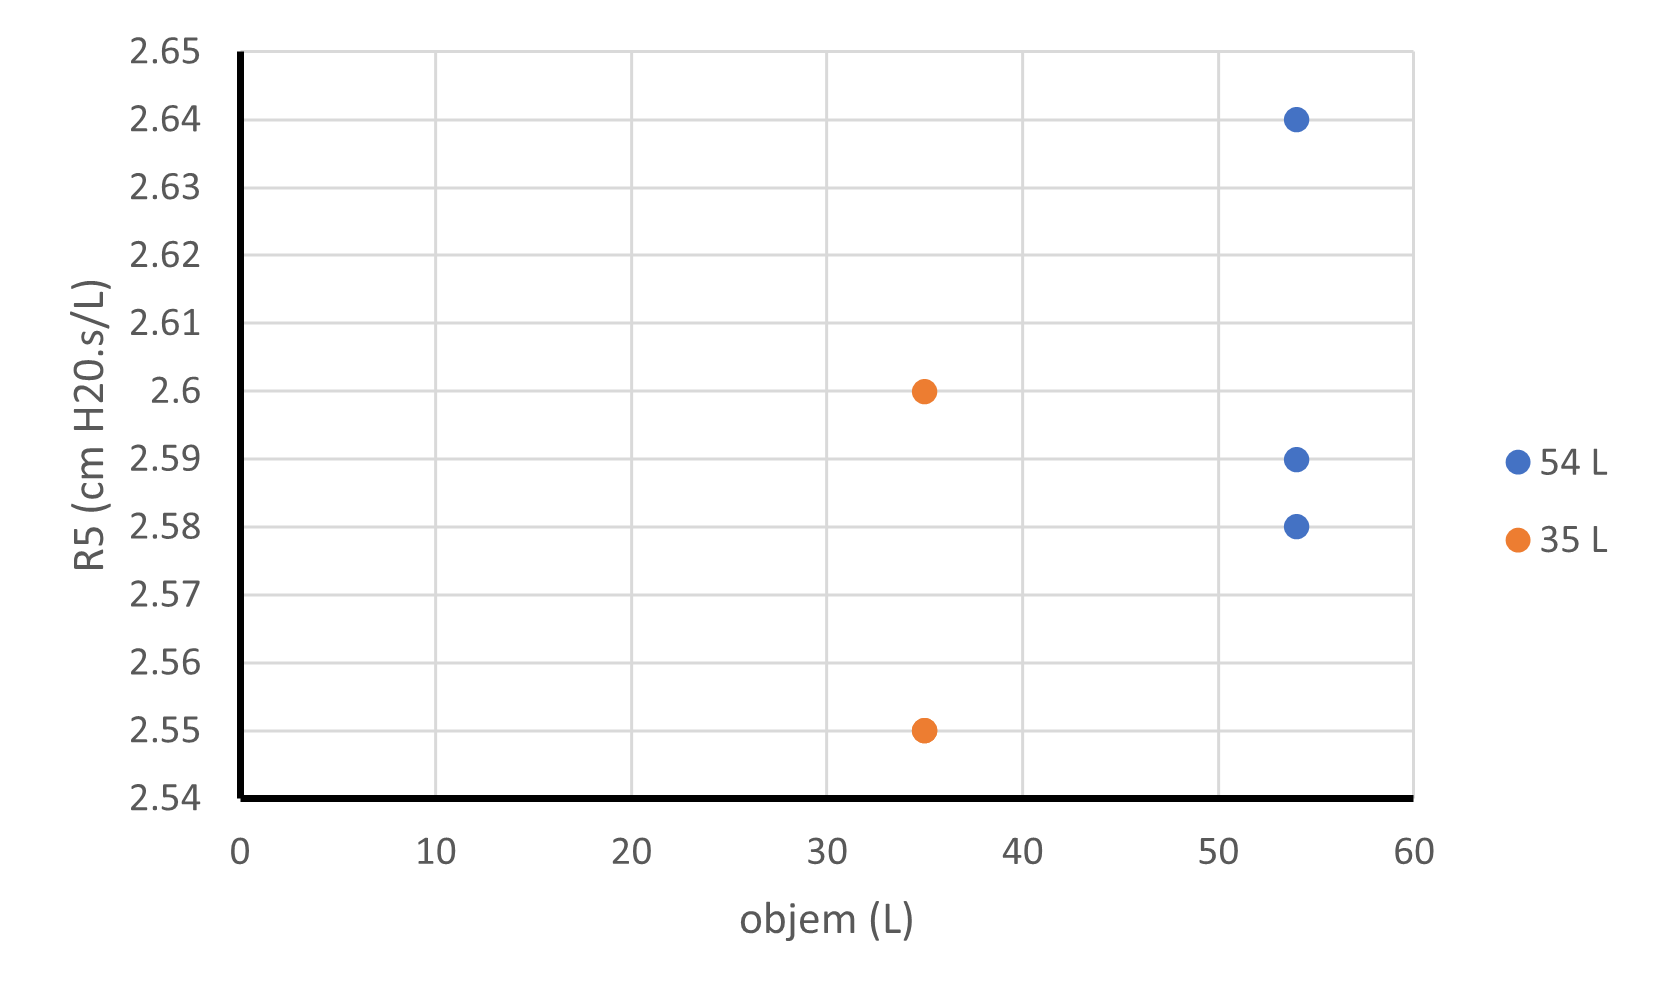
\includegraphics[width=1\textwidth]{rezistance_odpor_50_delka_20_cm}
		\caption{Délka \SI{20}{cm}, odpor~50}
	\end{center}
\end{figure}

\begin{figure}[ht]
	\label{img:pic_rezistance_odpor_50_delka_40_cm}
	\begin{center}
		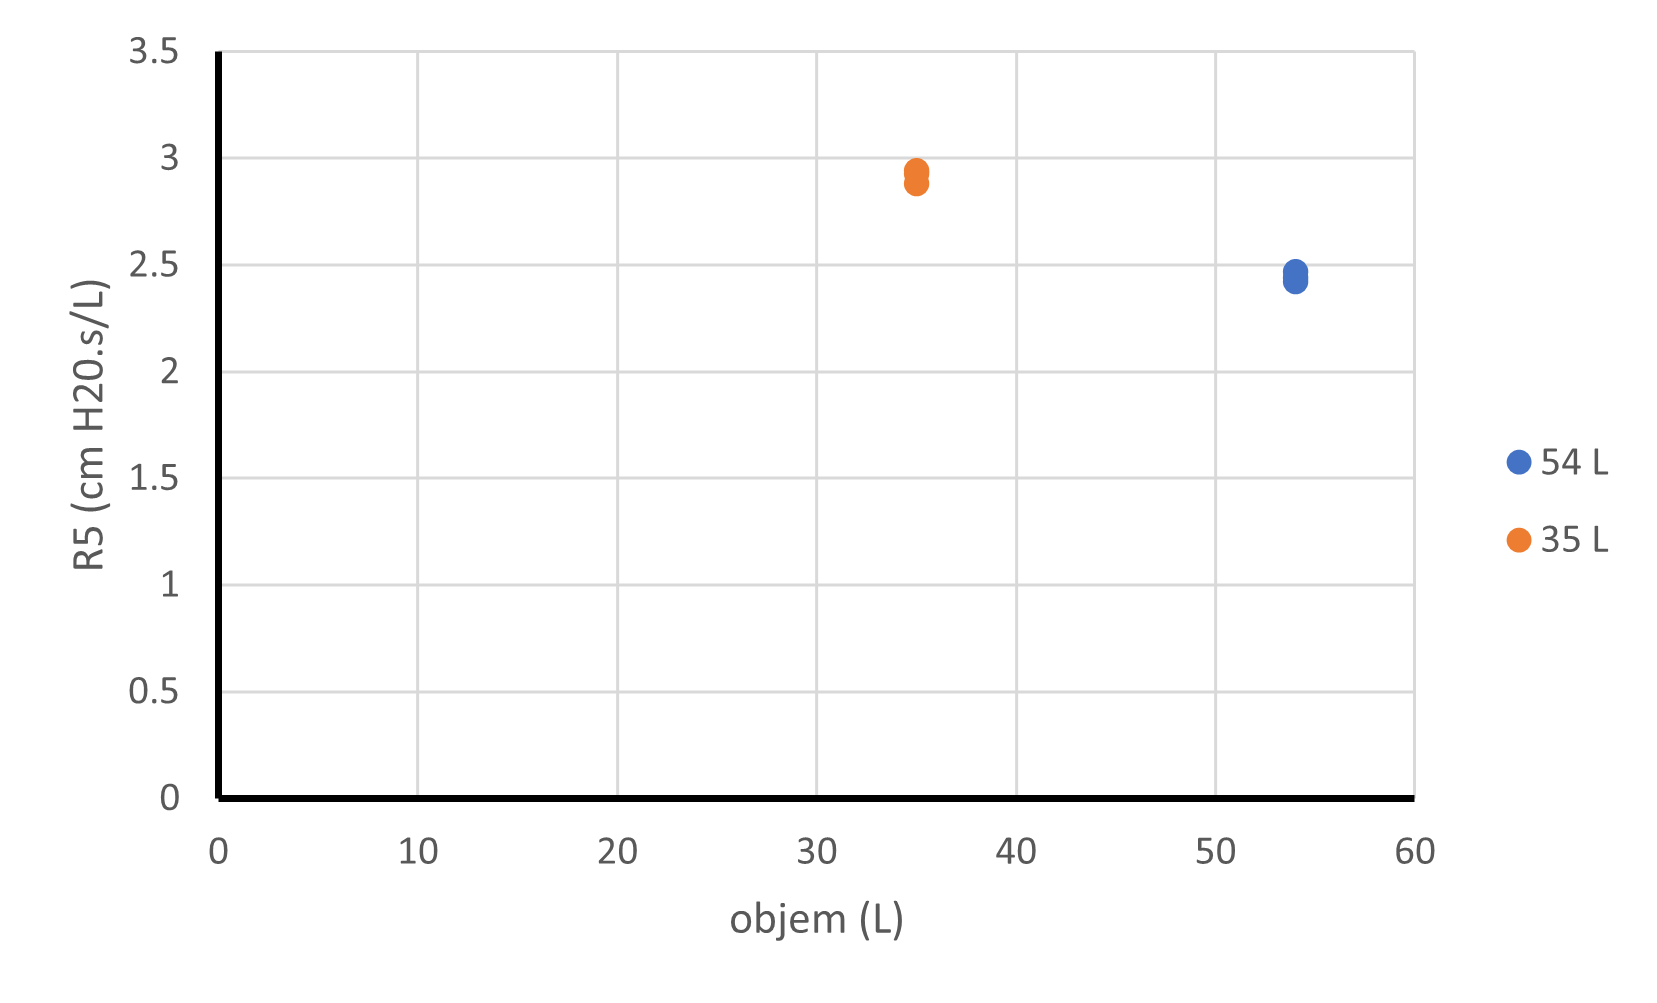
\includegraphics[width=1\textwidth]{rezistance_odpor_50_delka_40_cm}
		\caption{Délka \SI{40}{cm}, odpor~50}
	\end{center}
\end{figure}

\begin{figure}[ht]
	\label{img:pic_rezistance_odpor_5_nadoba_35_L}
	\begin{center}
		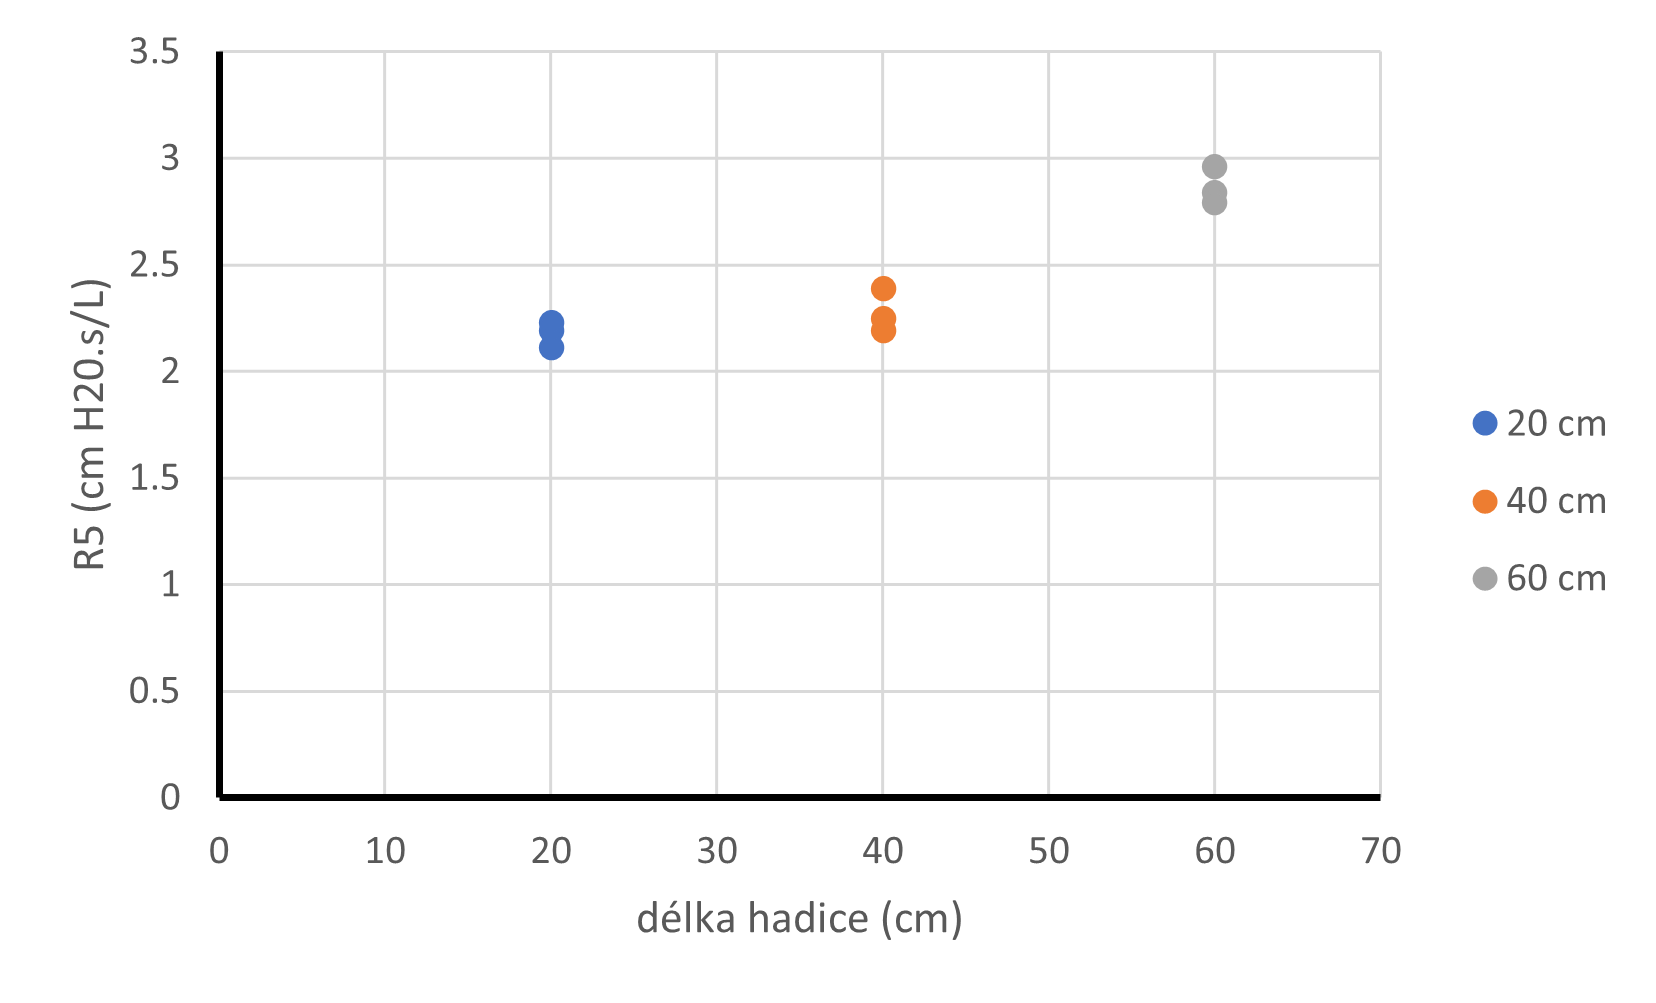
\includegraphics[width=1\textwidth]{rezistance_odpor_5_nadoba_35_L}
		\caption{Nádoba \SI{35}{L}, odpor~5}
	\end{center}
\end{figure}

\begin{figure}[ht]
	\label{img:pic_rezistance_odpor_5_nadoba_54_L}
	\begin{center}
		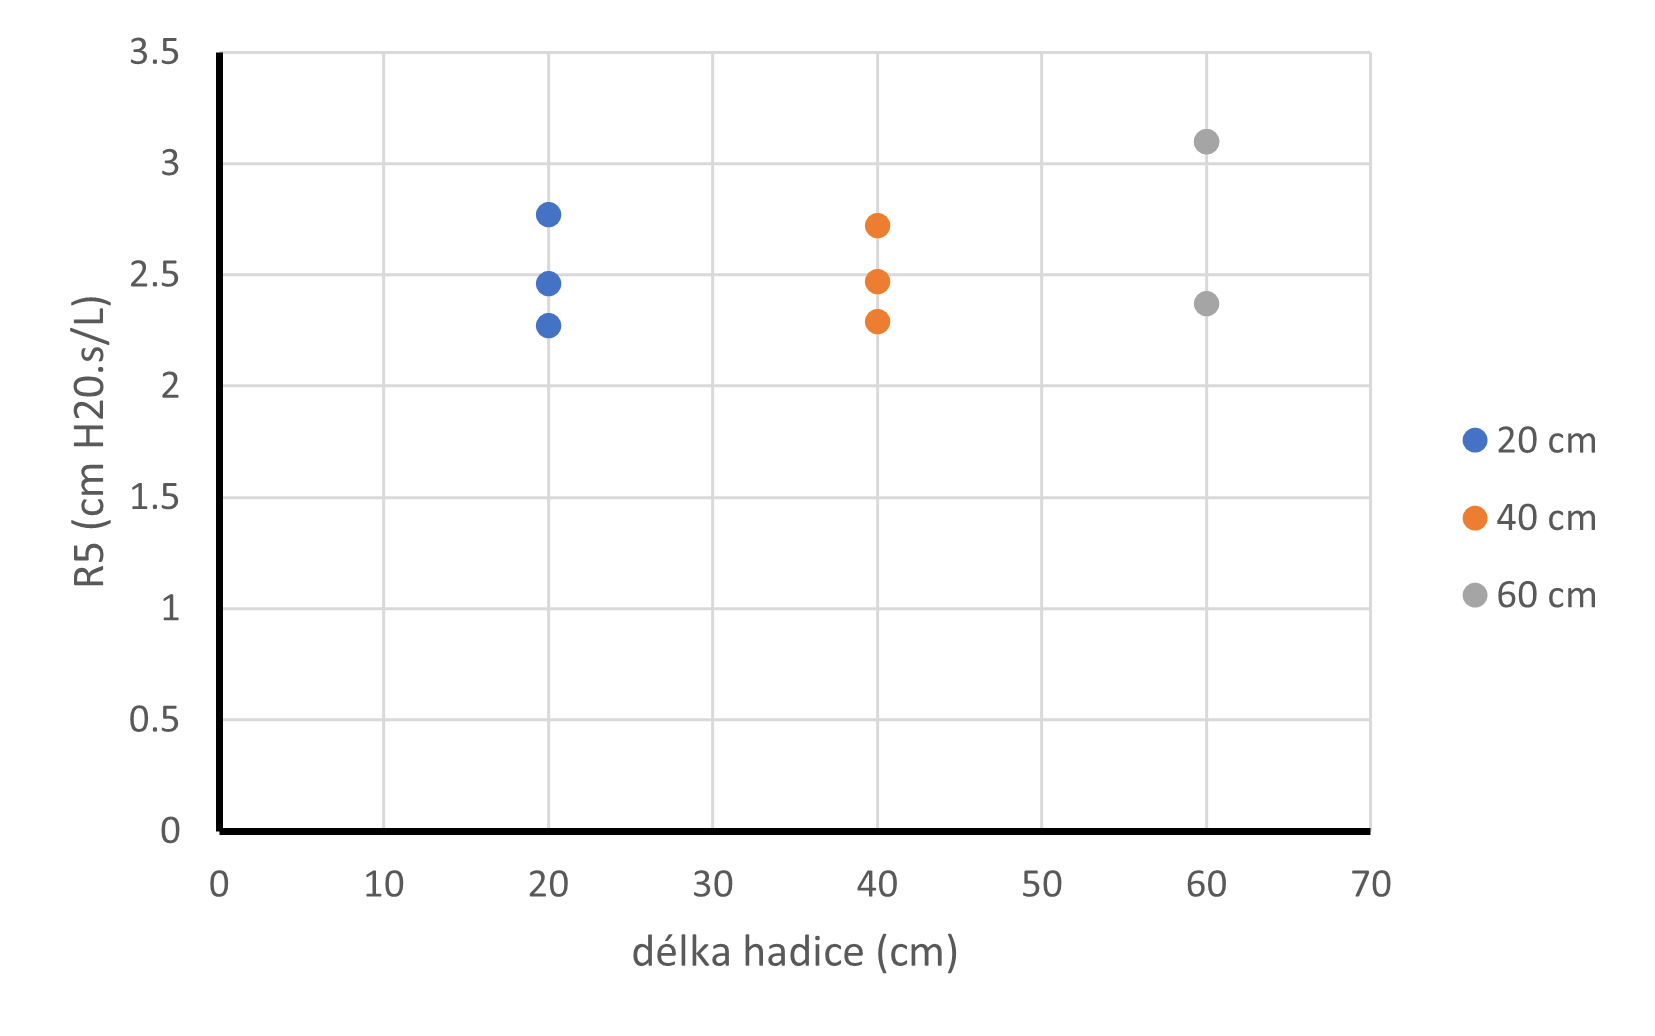
\includegraphics[width=1\textwidth]{rezistance_odpor_5_nadoba_54_L}
		\caption{Nádoba \SI{54}{L}, odpor~5}
	\end{center}
\end{figure}

\begin{figure}[ht]
	\label{img:pic_rezistance_odpor_20_nadoba_35_L}
	\begin{center}
		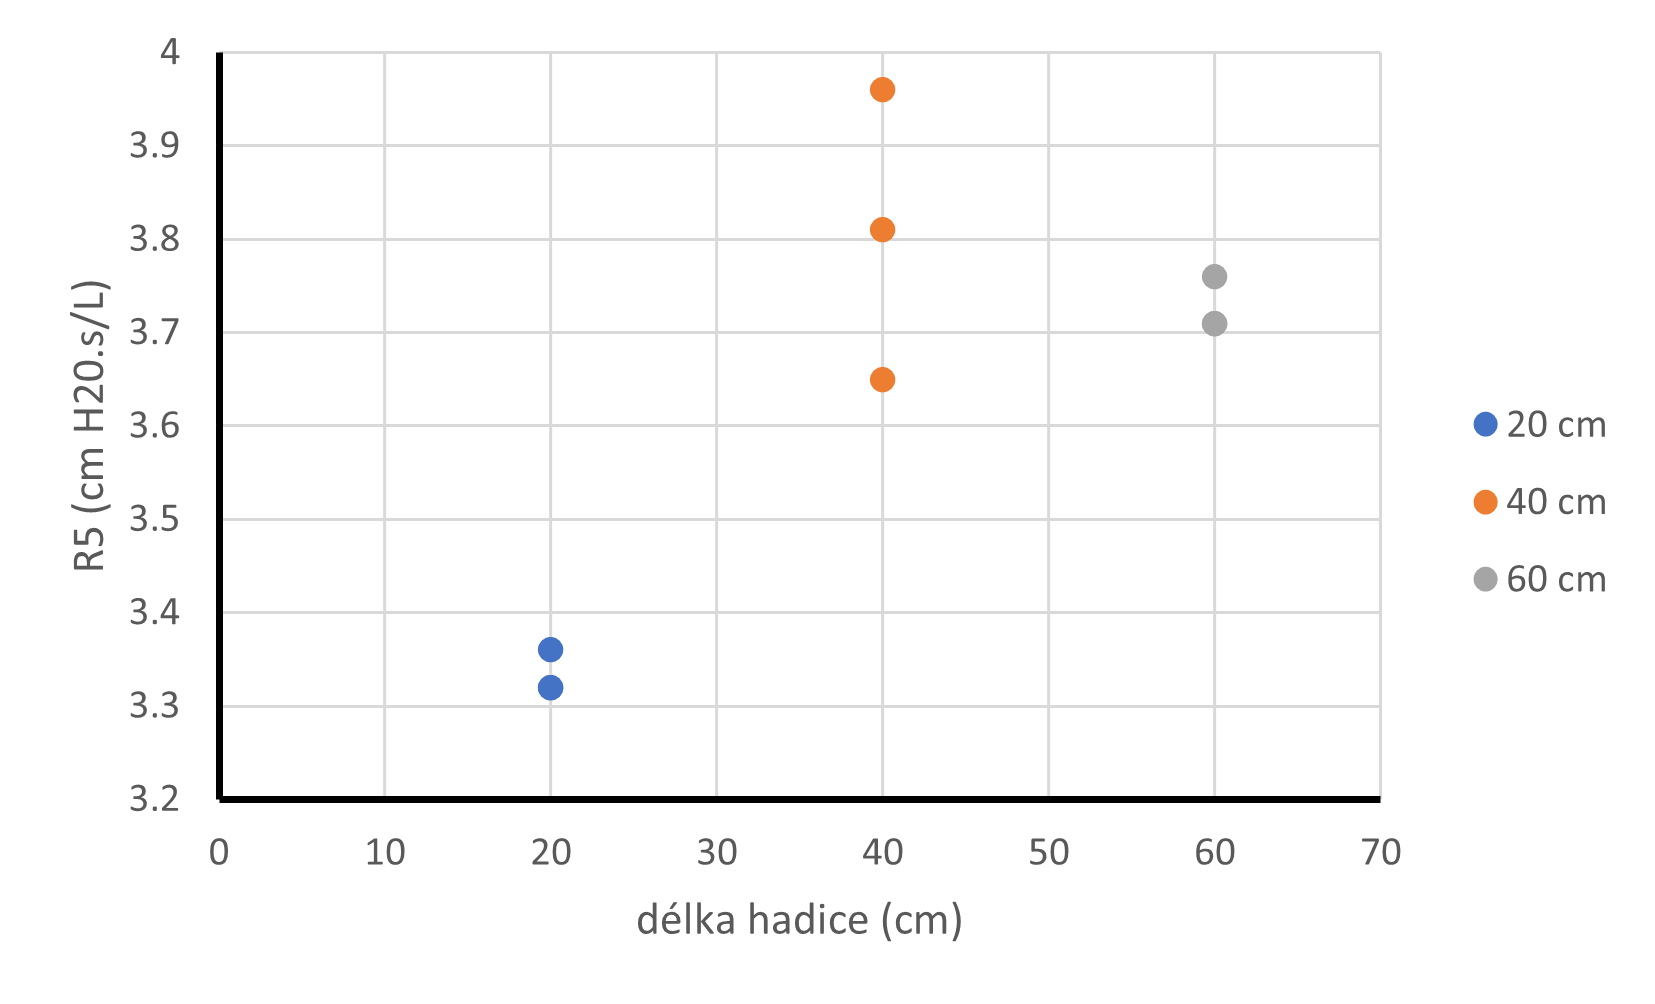
\includegraphics[width=1\textwidth]{rezistance_odpor_20_nadoba_35_L}
		\caption{Nádoba \SI{35}{L}, odpor~20}
	\end{center}
\end{figure}

\begin{figure}[ht]
	\label{img:pic_rezistance_odpor_20_nadoba_54_L}
	\begin{center}
		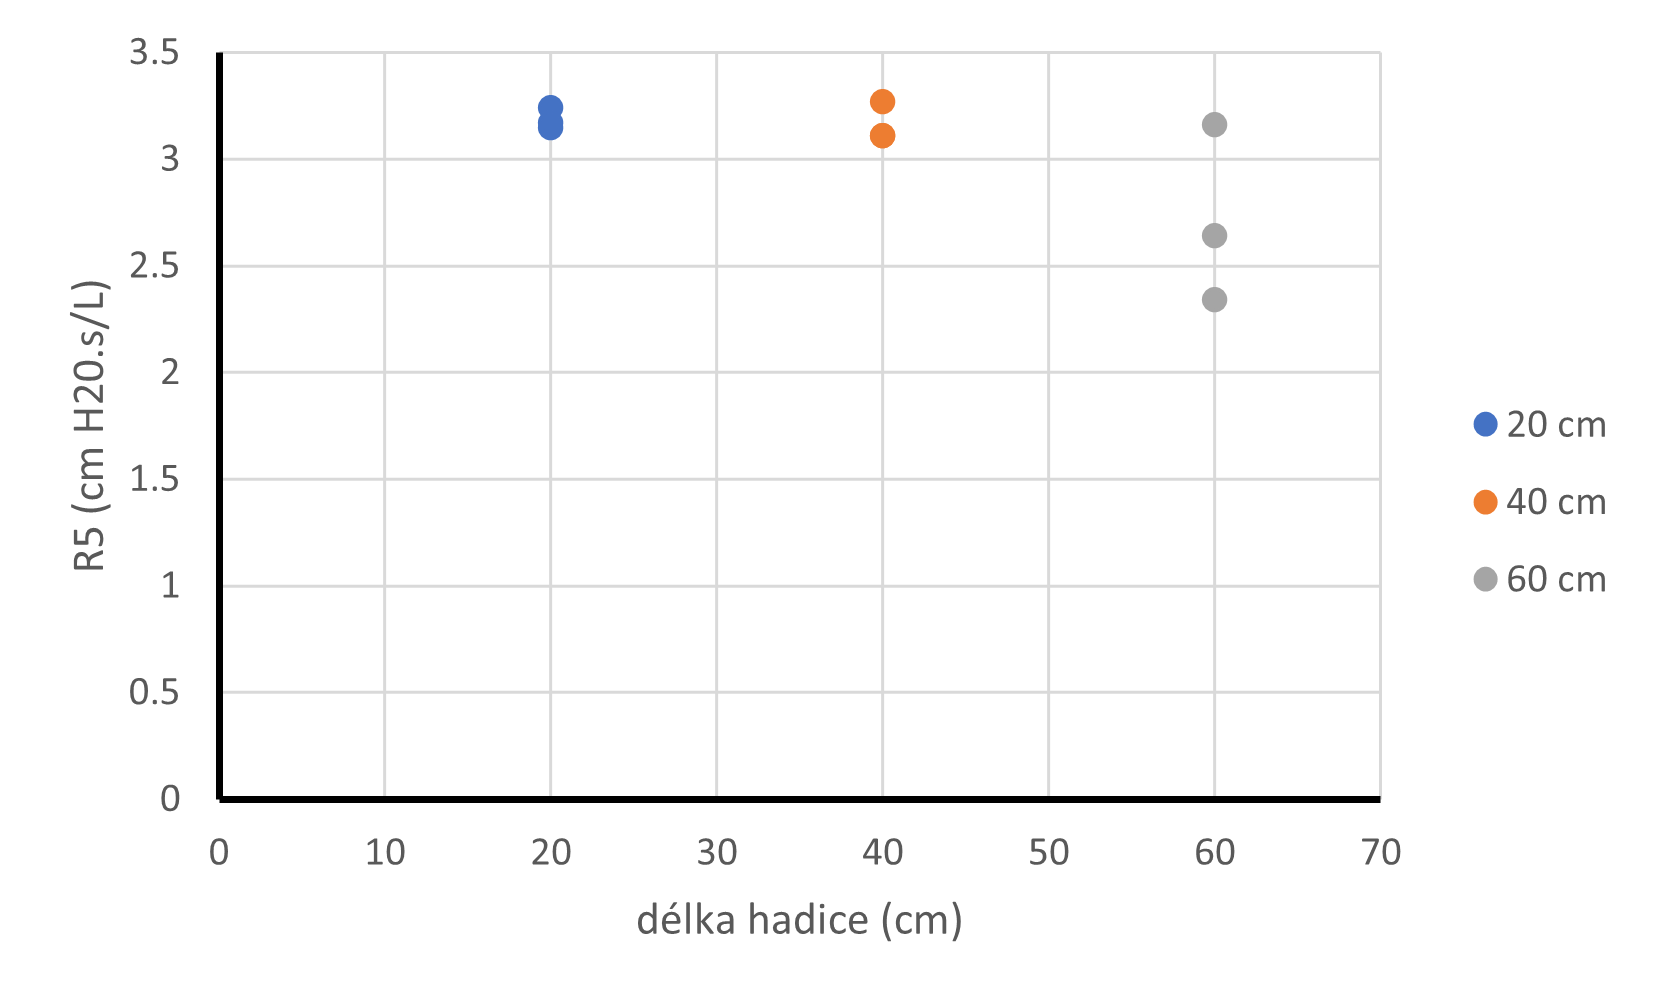
\includegraphics[width=1\textwidth]{rezistance_odpor_20_nadoba_54_L}
		\caption{Nádoba \SI{54}{L}, odpor~20}
	\end{center}
\end{figure}

\begin{figure}[ht]
	\label{img:pic_rezistance_odpor_50_nadoba_35_L}
	\begin{center}
		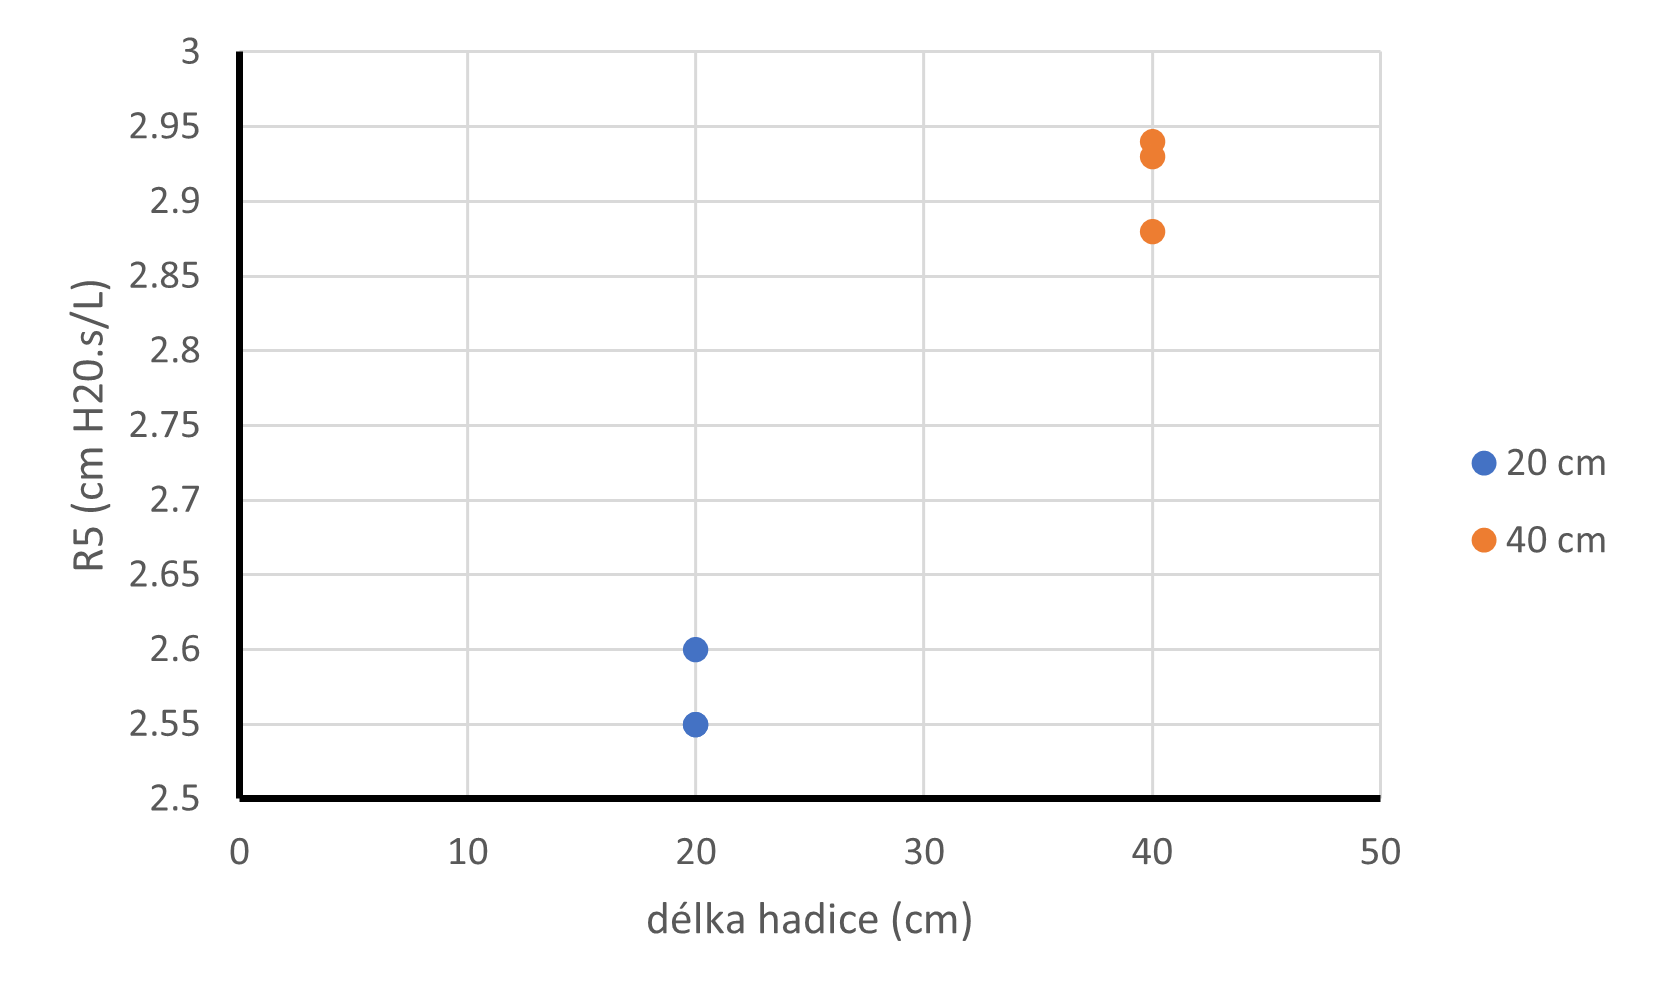
\includegraphics[width=1\textwidth]{rezistance_odpor_50_nadoba_35_L}
		\caption{Nádoba \SI{35}{L}, odpor~50}
	\end{center}
\end{figure}

\begin{figure}[ht]
	\label{img:pic_rezistance_odpor_50_nadoba_54_L}
	\begin{center}
		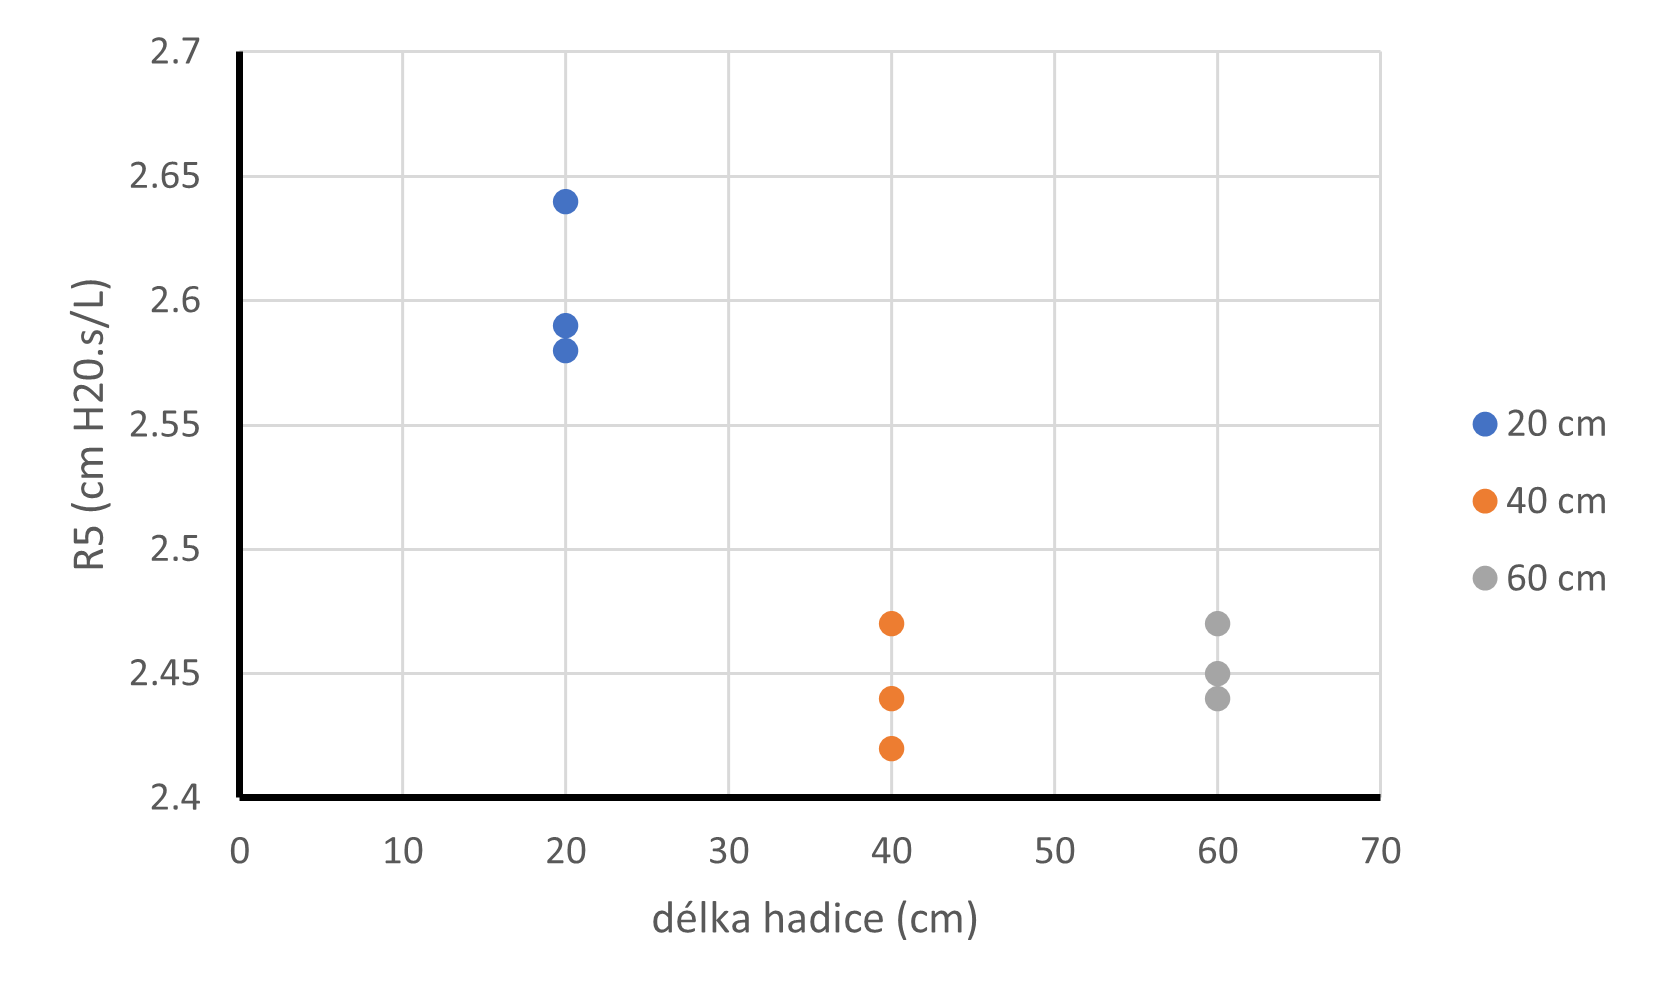
\includegraphics[width=1\textwidth]{rezistance_odpor_50_nadoba_54_L}
		\caption{Nádoba \SI{54}{L}, odpor~50}
	\end{center}
\end{figure}
